% Created by tikzDevice version 0.6.2-92-0ad2792 on 2013-03-06 20:12:02
% !TEX encoding = UTF-8 Unicode
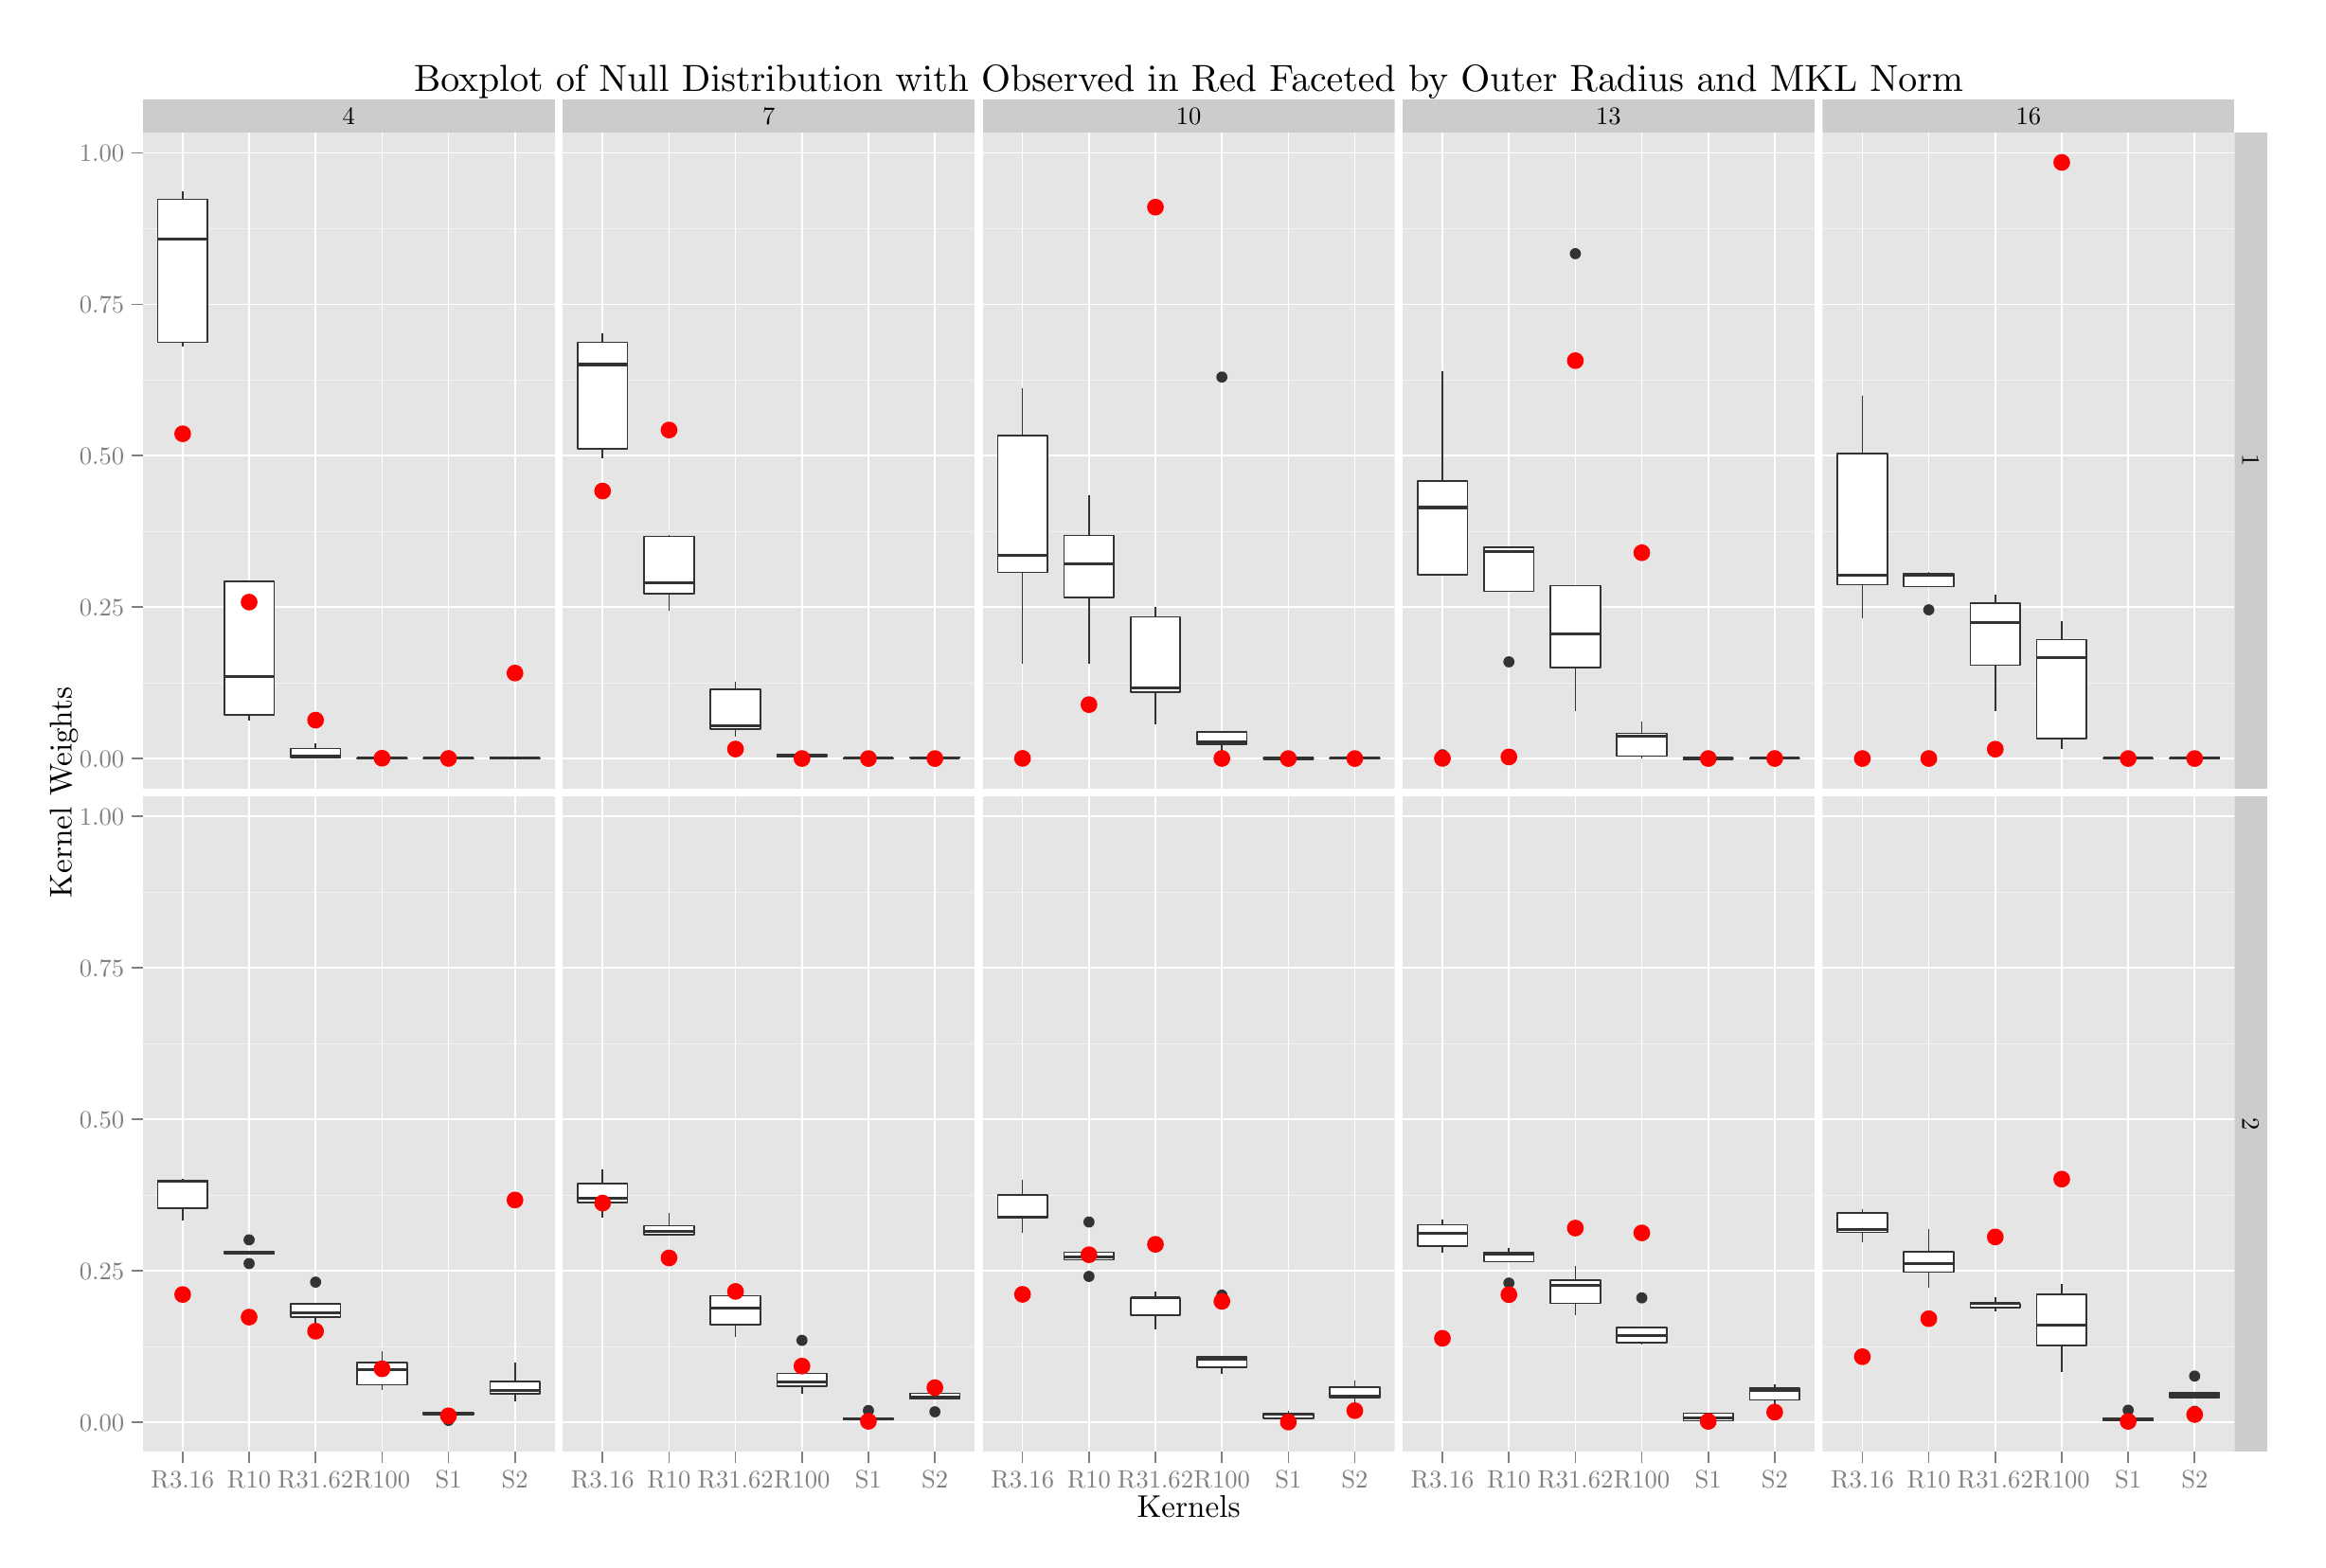
\begin{tikzpicture}[x=1pt,y=1pt]
\definecolor[named]{fillColor}{rgb}{1.00,1.00,1.00}
\path[use as bounding box,fill=fillColor,fill opacity=0.00] (0,0) rectangle (867.24,578.16);
\begin{scope}
\path[clip] (  0.00,  0.00) rectangle (867.24,578.16);
\definecolor[named]{drawColor}{rgb}{1.00,1.00,1.00}
\definecolor[named]{fillColor}{rgb}{1.00,1.00,1.00}

\path[draw=drawColor,line width= 0.6pt,line join=round,line cap=round,fill=fillColor] ( -0.00,  0.00) rectangle (867.24,578.16);
\end{scope}
\begin{scope}
\path[clip] ( 44.49,537.54) rectangle (201.69,550.17);
\definecolor[named]{fillColor}{rgb}{0.80,0.80,0.80}

\path[fill=fillColor] ( 44.49,537.54) rectangle (201.69,550.17);
\definecolor[named]{drawColor}{rgb}{0.00,0.00,0.00}

\node[text=drawColor,anchor=base,inner sep=0pt, outer sep=0pt, scale=  0.96] at (123.09,540.55) {4};
\end{scope}
\begin{scope}
\path[clip] (204.70,537.54) rectangle (361.91,550.17);
\definecolor[named]{fillColor}{rgb}{0.80,0.80,0.80}

\path[fill=fillColor] (204.70,537.54) rectangle (361.91,550.17);
\definecolor[named]{drawColor}{rgb}{0.00,0.00,0.00}

\node[text=drawColor,anchor=base,inner sep=0pt, outer sep=0pt, scale=  0.96] at (283.31,540.55) {7};
\end{scope}
\begin{scope}
\path[clip] (364.92,537.54) rectangle (522.13,550.17);
\definecolor[named]{fillColor}{rgb}{0.80,0.80,0.80}

\path[fill=fillColor] (364.92,537.54) rectangle (522.13,550.17);
\definecolor[named]{drawColor}{rgb}{0.00,0.00,0.00}

\node[text=drawColor,anchor=base,inner sep=0pt, outer sep=0pt, scale=  0.96] at (443.52,540.55) {10};
\end{scope}
\begin{scope}
\path[clip] (525.14,537.54) rectangle (682.34,550.17);
\definecolor[named]{fillColor}{rgb}{0.80,0.80,0.80}

\path[fill=fillColor] (525.14,537.54) rectangle (682.34,550.17);
\definecolor[named]{drawColor}{rgb}{0.00,0.00,0.00}

\node[text=drawColor,anchor=base,inner sep=0pt, outer sep=0pt, scale=  0.96] at (603.74,540.55) {13};
\end{scope}
\begin{scope}
\path[clip] (685.35,537.54) rectangle (842.56,550.17);
\definecolor[named]{fillColor}{rgb}{0.80,0.80,0.80}

\path[fill=fillColor] (685.35,537.54) rectangle (842.56,550.17);
\definecolor[named]{drawColor}{rgb}{0.00,0.00,0.00}

\node[text=drawColor,anchor=base,inner sep=0pt, outer sep=0pt, scale=  0.96] at (763.96,540.55) {16};
\end{scope}
\begin{scope}
\path[clip] ( 44.49,287.29) rectangle (201.69,537.54);
\definecolor[named]{fillColor}{rgb}{0.90,0.90,0.90}

\path[fill=fillColor] ( 44.49,287.29) rectangle (201.69,537.54);
\definecolor[named]{drawColor}{rgb}{0.95,0.95,0.95}

\path[draw=drawColor,line width= 0.3pt,line join=round] ( 44.49,327.56) --
	(201.69,327.56);

\path[draw=drawColor,line width= 0.3pt,line join=round] ( 44.49,385.35) --
	(201.69,385.35);

\path[draw=drawColor,line width= 0.3pt,line join=round] ( 44.49,443.13) --
	(201.69,443.13);

\path[draw=drawColor,line width= 0.3pt,line join=round] ( 44.49,500.92) --
	(201.69,500.92);
\definecolor[named]{drawColor}{rgb}{1.00,1.00,1.00}

\path[draw=drawColor,line width= 0.6pt,line join=round] ( 44.49,298.66) --
	(201.69,298.66);

\path[draw=drawColor,line width= 0.6pt,line join=round] ( 44.49,356.45) --
	(201.69,356.45);

\path[draw=drawColor,line width= 0.6pt,line join=round] ( 44.49,414.24) --
	(201.69,414.24);

\path[draw=drawColor,line width= 0.6pt,line join=round] ( 44.49,472.03) --
	(201.69,472.03);

\path[draw=drawColor,line width= 0.6pt,line join=round] ( 44.49,529.82) --
	(201.69,529.82);

\path[draw=drawColor,line width= 0.6pt,line join=round] ( 59.70,287.29) --
	( 59.70,537.54);

\path[draw=drawColor,line width= 0.6pt,line join=round] ( 85.05,287.29) --
	( 85.05,537.54);

\path[draw=drawColor,line width= 0.6pt,line join=round] (110.41,287.29) --
	(110.41,537.54);

\path[draw=drawColor,line width= 0.6pt,line join=round] (135.77,287.29) --
	(135.77,537.54);

\path[draw=drawColor,line width= 0.6pt,line join=round] (161.12,287.29) --
	(161.12,537.54);

\path[draw=drawColor,line width= 0.6pt,line join=round] (186.48,287.29) --
	(186.48,537.54);
\definecolor[named]{drawColor}{rgb}{0.20,0.20,0.20}
\definecolor[named]{fillColor}{rgb}{0.20,0.20,0.20}

\path[draw=drawColor,line width= 0.6pt,line join=round,fill=fillColor] ( 59.70,512.09) -- ( 59.70,515.28);

\path[draw=drawColor,line width= 0.6pt,line join=round,fill=fillColor] ( 59.70,457.47) -- ( 59.70,455.76);
\definecolor[named]{fillColor}{rgb}{1.00,1.00,1.00}

\path[draw=drawColor,line width= 0.6pt,line join=round,line cap=round,fill=fillColor] ( 50.19,512.09) --
	( 50.19,457.47) --
	( 69.21,457.47) --
	( 69.21,512.09) --
	( 50.19,512.09) --
	cycle;
\definecolor[named]{fillColor}{rgb}{0.20,0.20,0.20}

\path[draw=drawColor,line width= 1.1pt,line join=round,fill=fillColor] ( 50.19,496.94) -- ( 69.21,496.94);

\path[draw=drawColor,line width= 0.6pt,line join=round,fill=fillColor] ( 85.05,366.32) -- ( 85.05,366.78);

\path[draw=drawColor,line width= 0.6pt,line join=round,fill=fillColor] ( 85.05,315.32) -- ( 85.05,313.09);
\definecolor[named]{fillColor}{rgb}{1.00,1.00,1.00}

\path[draw=drawColor,line width= 0.6pt,line join=round,line cap=round,fill=fillColor] ( 75.55,366.32) --
	( 75.55,315.32) --
	( 94.56,315.32) --
	( 94.56,366.32) --
	( 75.55,366.32) --
	cycle;
\definecolor[named]{fillColor}{rgb}{0.20,0.20,0.20}

\path[draw=drawColor,line width= 1.1pt,line join=round,fill=fillColor] ( 75.55,329.97) -- ( 94.56,329.97);

\path[draw=drawColor,line width= 0.6pt,line join=round,fill=fillColor] (110.41,302.49) -- (110.41,304.32);

\path[draw=drawColor,line width= 0.6pt,line join=round,fill=fillColor] (110.41,299.18) -- (110.41,298.72);
\definecolor[named]{fillColor}{rgb}{1.00,1.00,1.00}

\path[draw=drawColor,line width= 0.6pt,line join=round,line cap=round,fill=fillColor] (100.90,302.49) --
	(100.90,299.18) --
	(119.92,299.18) --
	(119.92,302.49) --
	(100.90,302.49) --
	cycle;
\definecolor[named]{fillColor}{rgb}{0.20,0.20,0.20}

\path[draw=drawColor,line width= 1.1pt,line join=round,fill=fillColor] (100.90,299.66) -- (119.92,299.66);

\path[fill=fillColor] (135.77,298.69) circle (  2.13);

\path[fill=fillColor] (135.77,298.95) circle (  2.13);

\path[draw=drawColor,line width= 0.6pt,line join=round,fill=fillColor] (135.77,298.83) -- (135.77,298.83);

\path[draw=drawColor,line width= 0.6pt,line join=round,fill=fillColor] (135.77,298.81) -- (135.77,298.81);
\definecolor[named]{fillColor}{rgb}{1.00,1.00,1.00}

\path[draw=drawColor,line width= 0.6pt,line join=round,line cap=round,fill=fillColor] (126.26,298.83) --
	(126.26,298.81) --
	(145.27,298.81) --
	(145.27,298.83) --
	(126.26,298.83) --
	cycle;
\definecolor[named]{fillColor}{rgb}{0.20,0.20,0.20}

\path[draw=drawColor,line width= 1.1pt,line join=round,fill=fillColor] (126.26,298.83) -- (145.27,298.83);

\path[fill=fillColor] (161.12,298.68) circle (  2.13);

\path[draw=drawColor,line width= 0.6pt,line join=round,fill=fillColor] (161.12,298.82) -- (161.12,298.86);

\path[draw=drawColor,line width= 0.6pt,line join=round,fill=fillColor] (161.12,298.76) -- (161.12,298.76);
\definecolor[named]{fillColor}{rgb}{1.00,1.00,1.00}

\path[draw=drawColor,line width= 0.6pt,line join=round,line cap=round,fill=fillColor] (151.61,298.82) --
	(151.61,298.76) --
	(170.63,298.76) --
	(170.63,298.82) --
	(151.61,298.82) --
	cycle;
\definecolor[named]{fillColor}{rgb}{0.20,0.20,0.20}

\path[draw=drawColor,line width= 1.1pt,line join=round,fill=fillColor] (151.61,298.80) -- (170.63,298.80);

\path[draw=drawColor,line width= 0.6pt,line join=round,fill=fillColor] (186.48,298.92) -- (186.48,298.93);

\path[draw=drawColor,line width= 0.6pt,line join=round,fill=fillColor] (186.48,298.80) -- (186.48,298.68);
\definecolor[named]{fillColor}{rgb}{1.00,1.00,1.00}

\path[draw=drawColor,line width= 0.6pt,line join=round,line cap=round,fill=fillColor] (176.97,298.92) --
	(176.97,298.80) --
	(195.99,298.80) --
	(195.99,298.92) --
	(176.97,298.92) --
	cycle;
\definecolor[named]{fillColor}{rgb}{0.20,0.20,0.20}

\path[draw=drawColor,line width= 1.1pt,line join=round,fill=fillColor] (176.97,298.91) -- (195.99,298.91);
\definecolor[named]{fillColor}{rgb}{1.00,0.00,0.00}

\path[fill=fillColor] ( 59.70,422.61) circle (  3.20);

\path[fill=fillColor] ( 85.05,358.37) circle (  3.20);

\path[fill=fillColor] (110.41,313.34) circle (  3.20);

\path[fill=fillColor] (135.77,298.80) circle (  3.20);

\path[fill=fillColor] (161.12,298.71) circle (  3.20);

\path[fill=fillColor] (186.48,331.30) circle (  3.20);
\end{scope}
\begin{scope}
\path[clip] ( 44.49, 34.03) rectangle (201.69,284.28);
\definecolor[named]{fillColor}{rgb}{0.90,0.90,0.90}

\path[fill=fillColor] ( 44.49, 34.03) rectangle (201.69,284.28);
\definecolor[named]{drawColor}{rgb}{0.95,0.95,0.95}

\path[draw=drawColor,line width= 0.3pt,line join=round] ( 44.49, 74.30) --
	(201.69, 74.30);

\path[draw=drawColor,line width= 0.3pt,line join=round] ( 44.49,132.09) --
	(201.69,132.09);

\path[draw=drawColor,line width= 0.3pt,line join=round] ( 44.49,189.88) --
	(201.69,189.88);

\path[draw=drawColor,line width= 0.3pt,line join=round] ( 44.49,247.66) --
	(201.69,247.66);
\definecolor[named]{drawColor}{rgb}{1.00,1.00,1.00}

\path[draw=drawColor,line width= 0.6pt,line join=round] ( 44.49, 45.41) --
	(201.69, 45.41);

\path[draw=drawColor,line width= 0.6pt,line join=round] ( 44.49,103.19) --
	(201.69,103.19);

\path[draw=drawColor,line width= 0.6pt,line join=round] ( 44.49,160.98) --
	(201.69,160.98);

\path[draw=drawColor,line width= 0.6pt,line join=round] ( 44.49,218.77) --
	(201.69,218.77);

\path[draw=drawColor,line width= 0.6pt,line join=round] ( 44.49,276.56) --
	(201.69,276.56);

\path[draw=drawColor,line width= 0.6pt,line join=round] ( 59.70, 34.03) --
	( 59.70,284.28);

\path[draw=drawColor,line width= 0.6pt,line join=round] ( 85.05, 34.03) --
	( 85.05,284.28);

\path[draw=drawColor,line width= 0.6pt,line join=round] (110.41, 34.03) --
	(110.41,284.28);

\path[draw=drawColor,line width= 0.6pt,line join=round] (135.77, 34.03) --
	(135.77,284.28);

\path[draw=drawColor,line width= 0.6pt,line join=round] (161.12, 34.03) --
	(161.12,284.28);

\path[draw=drawColor,line width= 0.6pt,line join=round] (186.48, 34.03) --
	(186.48,284.28);
\definecolor[named]{drawColor}{rgb}{0.20,0.20,0.20}
\definecolor[named]{fillColor}{rgb}{0.20,0.20,0.20}

\path[draw=drawColor,line width= 0.6pt,line join=round,fill=fillColor] ( 59.70,137.72) -- ( 59.70,138.18);

\path[draw=drawColor,line width= 0.6pt,line join=round,fill=fillColor] ( 59.70,127.10) -- ( 59.70,122.43);
\definecolor[named]{fillColor}{rgb}{1.00,1.00,1.00}

\path[draw=drawColor,line width= 0.6pt,line join=round,line cap=round,fill=fillColor] ( 50.19,137.72) --
	( 50.19,127.10) --
	( 69.21,127.10) --
	( 69.21,137.72) --
	( 50.19,137.72) --
	cycle;
\definecolor[named]{fillColor}{rgb}{0.20,0.20,0.20}

\path[draw=drawColor,line width= 1.1pt,line join=round,fill=fillColor] ( 50.19,137.25) -- ( 69.21,137.25);

\path[fill=fillColor] ( 85.05,105.95) circle (  2.13);

\path[fill=fillColor] ( 85.05,115.00) circle (  2.13);

\path[draw=drawColor,line width= 0.6pt,line join=round,fill=fillColor] ( 85.05,110.39) -- ( 85.05,110.39);

\path[draw=drawColor,line width= 0.6pt,line join=round,fill=fillColor] ( 85.05,109.66) -- ( 85.05,109.66);
\definecolor[named]{fillColor}{rgb}{1.00,1.00,1.00}

\path[draw=drawColor,line width= 0.6pt,line join=round,line cap=round,fill=fillColor] ( 75.55,110.39) --
	( 75.55,109.66) --
	( 94.56,109.66) --
	( 94.56,110.39) --
	( 75.55,110.39) --
	cycle;
\definecolor[named]{fillColor}{rgb}{0.20,0.20,0.20}

\path[draw=drawColor,line width= 1.1pt,line join=round,fill=fillColor] ( 75.55,110.23) -- ( 94.56,110.23);

\path[fill=fillColor] (110.41, 98.86) circle (  2.13);

\path[draw=drawColor,line width= 0.6pt,line join=round,fill=fillColor] (110.41, 90.60) -- (110.41, 90.60);

\path[draw=drawColor,line width= 0.6pt,line join=round,fill=fillColor] (110.41, 85.50) -- (110.41, 80.23);
\definecolor[named]{fillColor}{rgb}{1.00,1.00,1.00}

\path[draw=drawColor,line width= 0.6pt,line join=round,line cap=round,fill=fillColor] (100.90, 90.60) --
	(100.90, 85.50) --
	(119.92, 85.50) --
	(119.92, 90.60) --
	(100.90, 90.60) --
	cycle;
\definecolor[named]{fillColor}{rgb}{0.20,0.20,0.20}

\path[draw=drawColor,line width= 1.1pt,line join=round,fill=fillColor] (100.90, 87.04) -- (119.92, 87.04);

\path[draw=drawColor,line width= 0.6pt,line join=round,fill=fillColor] (135.77, 68.26) -- (135.77, 72.61);

\path[draw=drawColor,line width= 0.6pt,line join=round,fill=fillColor] (135.77, 59.65) -- (135.77, 57.70);
\definecolor[named]{fillColor}{rgb}{1.00,1.00,1.00}

\path[draw=drawColor,line width= 0.6pt,line join=round,line cap=round,fill=fillColor] (126.26, 68.26) --
	(126.26, 59.65) --
	(145.27, 59.65) --
	(145.27, 68.26) --
	(126.26, 68.26) --
	cycle;
\definecolor[named]{fillColor}{rgb}{0.20,0.20,0.20}

\path[draw=drawColor,line width= 1.1pt,line join=round,fill=fillColor] (126.26, 65.55) -- (145.27, 65.55);

\path[fill=fillColor] (161.12, 46.09) circle (  2.13);

\path[draw=drawColor,line width= 0.6pt,line join=round,fill=fillColor] (161.12, 49.08) -- (161.12, 49.68);

\path[draw=drawColor,line width= 0.6pt,line join=round,fill=fillColor] (161.12, 48.19) -- (161.12, 48.19);
\definecolor[named]{fillColor}{rgb}{1.00,1.00,1.00}

\path[draw=drawColor,line width= 0.6pt,line join=round,line cap=round,fill=fillColor] (151.61, 49.08) --
	(151.61, 48.19) --
	(170.63, 48.19) --
	(170.63, 49.08) --
	(151.61, 49.08) --
	cycle;
\definecolor[named]{fillColor}{rgb}{0.20,0.20,0.20}

\path[draw=drawColor,line width= 1.1pt,line join=round,fill=fillColor] (151.61, 48.92) -- (170.63, 48.92);

\path[draw=drawColor,line width= 0.6pt,line join=round,fill=fillColor] (186.48, 60.99) -- (186.48, 68.00);

\path[draw=drawColor,line width= 0.6pt,line join=round,fill=fillColor] (186.48, 56.17) -- (186.48, 53.36);
\definecolor[named]{fillColor}{rgb}{1.00,1.00,1.00}

\path[draw=drawColor,line width= 0.6pt,line join=round,line cap=round,fill=fillColor] (176.97, 60.99) --
	(176.97, 56.17) --
	(195.99, 56.17) --
	(195.99, 60.99) --
	(176.97, 60.99) --
	cycle;
\definecolor[named]{fillColor}{rgb}{0.20,0.20,0.20}

\path[draw=drawColor,line width= 1.1pt,line join=round,fill=fillColor] (176.97, 57.52) -- (195.99, 57.52);
\definecolor[named]{fillColor}{rgb}{1.00,0.00,0.00}

\path[fill=fillColor] ( 59.70, 94.13) circle (  3.20);

\path[fill=fillColor] ( 85.05, 85.51) circle (  3.20);

\path[fill=fillColor] (110.41, 80.13) circle (  3.20);

\path[fill=fillColor] (135.77, 65.78) circle (  3.20);

\path[fill=fillColor] (161.12, 47.83) circle (  3.20);

\path[fill=fillColor] (186.48,130.20) circle (  3.20);
\end{scope}
\begin{scope}
\path[clip] (204.70,287.29) rectangle (361.91,537.54);
\definecolor[named]{fillColor}{rgb}{0.90,0.90,0.90}

\path[fill=fillColor] (204.70,287.29) rectangle (361.91,537.54);
\definecolor[named]{drawColor}{rgb}{0.95,0.95,0.95}

\path[draw=drawColor,line width= 0.3pt,line join=round] (204.70,327.56) --
	(361.91,327.56);

\path[draw=drawColor,line width= 0.3pt,line join=round] (204.70,385.35) --
	(361.91,385.35);

\path[draw=drawColor,line width= 0.3pt,line join=round] (204.70,443.13) --
	(361.91,443.13);

\path[draw=drawColor,line width= 0.3pt,line join=round] (204.70,500.92) --
	(361.91,500.92);
\definecolor[named]{drawColor}{rgb}{1.00,1.00,1.00}

\path[draw=drawColor,line width= 0.6pt,line join=round] (204.70,298.66) --
	(361.91,298.66);

\path[draw=drawColor,line width= 0.6pt,line join=round] (204.70,356.45) --
	(361.91,356.45);

\path[draw=drawColor,line width= 0.6pt,line join=round] (204.70,414.24) --
	(361.91,414.24);

\path[draw=drawColor,line width= 0.6pt,line join=round] (204.70,472.03) --
	(361.91,472.03);

\path[draw=drawColor,line width= 0.6pt,line join=round] (204.70,529.82) --
	(361.91,529.82);

\path[draw=drawColor,line width= 0.6pt,line join=round] (219.92,287.29) --
	(219.92,537.54);

\path[draw=drawColor,line width= 0.6pt,line join=round] (245.27,287.29) --
	(245.27,537.54);

\path[draw=drawColor,line width= 0.6pt,line join=round] (270.63,287.29) --
	(270.63,537.54);

\path[draw=drawColor,line width= 0.6pt,line join=round] (295.98,287.29) --
	(295.98,537.54);

\path[draw=drawColor,line width= 0.6pt,line join=round] (321.34,287.29) --
	(321.34,537.54);

\path[draw=drawColor,line width= 0.6pt,line join=round] (346.70,287.29) --
	(346.70,537.54);
\definecolor[named]{drawColor}{rgb}{0.20,0.20,0.20}
\definecolor[named]{fillColor}{rgb}{0.20,0.20,0.20}

\path[draw=drawColor,line width= 0.6pt,line join=round,fill=fillColor] (219.92,457.47) -- (219.92,461.08);

\path[draw=drawColor,line width= 0.6pt,line join=round,fill=fillColor] (219.92,416.93) -- (219.92,413.27);
\definecolor[named]{fillColor}{rgb}{1.00,1.00,1.00}

\path[draw=drawColor,line width= 0.6pt,line join=round,line cap=round,fill=fillColor] (210.41,457.47) --
	(210.41,416.93) --
	(229.42,416.93) --
	(229.42,457.47) --
	(210.41,457.47) --
	cycle;
\definecolor[named]{fillColor}{rgb}{0.20,0.20,0.20}

\path[draw=drawColor,line width= 1.1pt,line join=round,fill=fillColor] (210.41,449.04) -- (229.42,449.04);

\path[draw=drawColor,line width= 0.6pt,line join=round,fill=fillColor] (245.27,383.48) -- (245.27,384.01);

\path[draw=drawColor,line width= 0.6pt,line join=round,fill=fillColor] (245.27,361.51) -- (245.27,354.91);
\definecolor[named]{fillColor}{rgb}{1.00,1.00,1.00}

\path[draw=drawColor,line width= 0.6pt,line join=round,line cap=round,fill=fillColor] (235.76,383.48) --
	(235.76,361.51) --
	(254.78,361.51) --
	(254.78,383.48) --
	(235.76,383.48) --
	cycle;
\definecolor[named]{fillColor}{rgb}{0.20,0.20,0.20}

\path[draw=drawColor,line width= 1.1pt,line join=round,fill=fillColor] (235.76,365.71) -- (254.78,365.71);

\path[draw=drawColor,line width= 0.6pt,line join=round,fill=fillColor] (270.63,325.12) -- (270.63,327.87);

\path[draw=drawColor,line width= 0.6pt,line join=round,fill=fillColor] (270.63,309.99) -- (270.63,306.97);
\definecolor[named]{fillColor}{rgb}{1.00,1.00,1.00}

\path[draw=drawColor,line width= 0.6pt,line join=round,line cap=round,fill=fillColor] (261.12,325.12) --
	(261.12,309.99) --
	(280.14,309.99) --
	(280.14,325.12) --
	(261.12,325.12) --
	cycle;
\definecolor[named]{fillColor}{rgb}{0.20,0.20,0.20}

\path[draw=drawColor,line width= 1.1pt,line join=round,fill=fillColor] (261.12,311.19) -- (280.14,311.19);

\path[draw=drawColor,line width= 0.6pt,line join=round,fill=fillColor] (295.98,300.06) -- (295.98,300.20);

\path[draw=drawColor,line width= 0.6pt,line join=round,fill=fillColor] (295.98,299.34) -- (295.98,299.19);
\definecolor[named]{fillColor}{rgb}{1.00,1.00,1.00}

\path[draw=drawColor,line width= 0.6pt,line join=round,line cap=round,fill=fillColor] (286.48,300.06) --
	(286.48,299.34) --
	(305.49,299.34) --
	(305.49,300.06) --
	(286.48,300.06) --
	cycle;
\definecolor[named]{fillColor}{rgb}{0.20,0.20,0.20}

\path[draw=drawColor,line width= 1.1pt,line join=round,fill=fillColor] (286.48,299.52) -- (305.49,299.52);

\path[draw=drawColor,line width= 0.6pt,line join=round,fill=fillColor] (321.34,298.85) -- (321.34,298.88);

\path[draw=drawColor,line width= 0.6pt,line join=round,fill=fillColor] (321.34,298.78) -- (321.34,298.72);
\definecolor[named]{fillColor}{rgb}{1.00,1.00,1.00}

\path[draw=drawColor,line width= 0.6pt,line join=round,line cap=round,fill=fillColor] (311.83,298.85) --
	(311.83,298.78) --
	(330.85,298.78) --
	(330.85,298.85) --
	(311.83,298.85) --
	cycle;
\definecolor[named]{fillColor}{rgb}{0.20,0.20,0.20}

\path[draw=drawColor,line width= 1.1pt,line join=round,fill=fillColor] (311.83,298.84) -- (330.85,298.84);

\path[draw=drawColor,line width= 0.6pt,line join=round,fill=fillColor] (346.70,298.99) -- (346.70,299.12);

\path[draw=drawColor,line width= 0.6pt,line join=round,fill=fillColor] (346.70,298.84) -- (346.70,298.81);
\definecolor[named]{fillColor}{rgb}{1.00,1.00,1.00}

\path[draw=drawColor,line width= 0.6pt,line join=round,line cap=round,fill=fillColor] (337.19,298.99) --
	(337.19,298.84) --
	(356.20,298.84) --
	(356.20,298.99) --
	(337.19,298.99) --
	cycle;
\definecolor[named]{fillColor}{rgb}{0.20,0.20,0.20}

\path[draw=drawColor,line width= 1.1pt,line join=round,fill=fillColor] (337.19,298.95) -- (356.20,298.95);
\definecolor[named]{fillColor}{rgb}{1.00,0.00,0.00}

\path[fill=fillColor] (219.92,400.77) circle (  3.20);

\path[fill=fillColor] (245.27,424.05) circle (  3.20);

\path[fill=fillColor] (270.63,302.30) circle (  3.20);

\path[fill=fillColor] (295.98,298.68) circle (  3.20);

\path[fill=fillColor] (321.34,298.67) circle (  3.20);

\path[fill=fillColor] (346.70,298.67) circle (  3.20);
\end{scope}
\begin{scope}
\path[clip] (204.70, 34.03) rectangle (361.91,284.28);
\definecolor[named]{fillColor}{rgb}{0.90,0.90,0.90}

\path[fill=fillColor] (204.70, 34.03) rectangle (361.91,284.28);
\definecolor[named]{drawColor}{rgb}{0.95,0.95,0.95}

\path[draw=drawColor,line width= 0.3pt,line join=round] (204.70, 74.30) --
	(361.91, 74.30);

\path[draw=drawColor,line width= 0.3pt,line join=round] (204.70,132.09) --
	(361.91,132.09);

\path[draw=drawColor,line width= 0.3pt,line join=round] (204.70,189.88) --
	(361.91,189.88);

\path[draw=drawColor,line width= 0.3pt,line join=round] (204.70,247.66) --
	(361.91,247.66);
\definecolor[named]{drawColor}{rgb}{1.00,1.00,1.00}

\path[draw=drawColor,line width= 0.6pt,line join=round] (204.70, 45.41) --
	(361.91, 45.41);

\path[draw=drawColor,line width= 0.6pt,line join=round] (204.70,103.19) --
	(361.91,103.19);

\path[draw=drawColor,line width= 0.6pt,line join=round] (204.70,160.98) --
	(361.91,160.98);

\path[draw=drawColor,line width= 0.6pt,line join=round] (204.70,218.77) --
	(361.91,218.77);

\path[draw=drawColor,line width= 0.6pt,line join=round] (204.70,276.56) --
	(361.91,276.56);

\path[draw=drawColor,line width= 0.6pt,line join=round] (219.92, 34.03) --
	(219.92,284.28);

\path[draw=drawColor,line width= 0.6pt,line join=round] (245.27, 34.03) --
	(245.27,284.28);

\path[draw=drawColor,line width= 0.6pt,line join=round] (270.63, 34.03) --
	(270.63,284.28);

\path[draw=drawColor,line width= 0.6pt,line join=round] (295.98, 34.03) --
	(295.98,284.28);

\path[draw=drawColor,line width= 0.6pt,line join=round] (321.34, 34.03) --
	(321.34,284.28);

\path[draw=drawColor,line width= 0.6pt,line join=round] (346.70, 34.03) --
	(346.70,284.28);
\definecolor[named]{drawColor}{rgb}{0.20,0.20,0.20}
\definecolor[named]{fillColor}{rgb}{0.20,0.20,0.20}

\path[draw=drawColor,line width= 0.6pt,line join=round,fill=fillColor] (219.92,136.57) -- (219.92,142.03);

\path[draw=drawColor,line width= 0.6pt,line join=round,fill=fillColor] (219.92,129.29) -- (219.92,123.50);
\definecolor[named]{fillColor}{rgb}{1.00,1.00,1.00}

\path[draw=drawColor,line width= 0.6pt,line join=round,line cap=round,fill=fillColor] (210.41,136.57) --
	(210.41,129.29) --
	(229.42,129.29) --
	(229.42,136.57) --
	(210.41,136.57) --
	cycle;
\definecolor[named]{fillColor}{rgb}{0.20,0.20,0.20}

\path[draw=drawColor,line width= 1.1pt,line join=round,fill=fillColor] (210.41,130.79) -- (229.42,130.79);

\path[fill=fillColor] (245.27,108.92) circle (  2.13);

\path[draw=drawColor,line width= 0.6pt,line join=round,fill=fillColor] (245.27,120.43) -- (245.27,125.32);

\path[draw=drawColor,line width= 0.6pt,line join=round,fill=fillColor] (245.27,117.06) -- (245.27,117.06);
\definecolor[named]{fillColor}{rgb}{1.00,1.00,1.00}

\path[draw=drawColor,line width= 0.6pt,line join=round,line cap=round,fill=fillColor] (235.76,120.43) --
	(235.76,117.06) --
	(254.78,117.06) --
	(254.78,120.43) --
	(235.76,120.43) --
	cycle;
\definecolor[named]{fillColor}{rgb}{0.20,0.20,0.20}

\path[draw=drawColor,line width= 1.1pt,line join=round,fill=fillColor] (235.76,118.27) -- (254.78,118.27);

\path[draw=drawColor,line width= 0.6pt,line join=round,fill=fillColor] (270.63, 93.62) -- (270.63, 95.88);

\path[draw=drawColor,line width= 0.6pt,line join=round,fill=fillColor] (270.63, 82.55) -- (270.63, 77.86);
\definecolor[named]{fillColor}{rgb}{1.00,1.00,1.00}

\path[draw=drawColor,line width= 0.6pt,line join=round,line cap=round,fill=fillColor] (261.12, 93.62) --
	(261.12, 82.55) --
	(280.14, 82.55) --
	(280.14, 93.62) --
	(261.12, 93.62) --
	cycle;
\definecolor[named]{fillColor}{rgb}{0.20,0.20,0.20}

\path[draw=drawColor,line width= 1.1pt,line join=round,fill=fillColor] (261.12, 88.80) -- (280.14, 88.80);

\path[fill=fillColor] (295.98, 76.64) circle (  2.13);

\path[draw=drawColor,line width= 0.6pt,line join=round,fill=fillColor] (295.98, 63.96) -- (295.98, 63.96);

\path[draw=drawColor,line width= 0.6pt,line join=round,fill=fillColor] (295.98, 59.14) -- (295.98, 56.41);
\definecolor[named]{fillColor}{rgb}{1.00,1.00,1.00}

\path[draw=drawColor,line width= 0.6pt,line join=round,line cap=round,fill=fillColor] (286.48, 63.96) --
	(286.48, 59.14) --
	(305.49, 59.14) --
	(305.49, 63.96) --
	(286.48, 63.96) --
	cycle;
\definecolor[named]{fillColor}{rgb}{0.20,0.20,0.20}

\path[draw=drawColor,line width= 1.1pt,line join=round,fill=fillColor] (286.48, 60.74) -- (305.49, 60.74);

\path[fill=fillColor] (321.34, 49.87) circle (  2.13);

\path[draw=drawColor,line width= 0.6pt,line join=round,fill=fillColor] (321.34, 47.05) -- (321.34, 47.05);

\path[draw=drawColor,line width= 0.6pt,line join=round,fill=fillColor] (321.34, 46.36) -- (321.34, 46.05);
\definecolor[named]{fillColor}{rgb}{1.00,1.00,1.00}

\path[draw=drawColor,line width= 0.6pt,line join=round,line cap=round,fill=fillColor] (311.83, 47.05) --
	(311.83, 46.36) --
	(330.85, 46.36) --
	(330.85, 47.05) --
	(311.83, 47.05) --
	cycle;
\definecolor[named]{fillColor}{rgb}{0.20,0.20,0.20}

\path[draw=drawColor,line width= 1.1pt,line join=round,fill=fillColor] (311.83, 46.76) -- (330.85, 46.76);

\path[fill=fillColor] (346.70, 49.38) circle (  2.13);

\path[draw=drawColor,line width= 0.6pt,line join=round,fill=fillColor] (346.70, 56.40) -- (346.70, 59.14);

\path[draw=drawColor,line width= 0.6pt,line join=round,fill=fillColor] (346.70, 54.28) -- (346.70, 54.28);
\definecolor[named]{fillColor}{rgb}{1.00,1.00,1.00}

\path[draw=drawColor,line width= 0.6pt,line join=round,line cap=round,fill=fillColor] (337.19, 56.40) --
	(337.19, 54.28) --
	(356.20, 54.28) --
	(356.20, 56.40) --
	(337.19, 56.40) --
	cycle;
\definecolor[named]{fillColor}{rgb}{0.20,0.20,0.20}

\path[draw=drawColor,line width= 1.1pt,line join=round,fill=fillColor] (337.19, 54.85) -- (356.20, 54.85);
\definecolor[named]{fillColor}{rgb}{1.00,0.00,0.00}

\path[fill=fillColor] (219.92,129.03) circle (  3.20);

\path[fill=fillColor] (245.27,108.10) circle (  3.20);

\path[fill=fillColor] (270.63, 95.31) circle (  3.20);

\path[fill=fillColor] (295.98, 66.81) circle (  3.20);

\path[fill=fillColor] (321.34, 45.74) circle (  3.20);

\path[fill=fillColor] (346.70, 58.59) circle (  3.20);
\end{scope}
\begin{scope}
\path[clip] (364.92,287.29) rectangle (522.13,537.54);
\definecolor[named]{fillColor}{rgb}{0.90,0.90,0.90}

\path[fill=fillColor] (364.92,287.29) rectangle (522.13,537.54);
\definecolor[named]{drawColor}{rgb}{0.95,0.95,0.95}

\path[draw=drawColor,line width= 0.3pt,line join=round] (364.92,327.56) --
	(522.13,327.56);

\path[draw=drawColor,line width= 0.3pt,line join=round] (364.92,385.35) --
	(522.13,385.35);

\path[draw=drawColor,line width= 0.3pt,line join=round] (364.92,443.13) --
	(522.13,443.13);

\path[draw=drawColor,line width= 0.3pt,line join=round] (364.92,500.92) --
	(522.13,500.92);
\definecolor[named]{drawColor}{rgb}{1.00,1.00,1.00}

\path[draw=drawColor,line width= 0.6pt,line join=round] (364.92,298.66) --
	(522.13,298.66);

\path[draw=drawColor,line width= 0.6pt,line join=round] (364.92,356.45) --
	(522.13,356.45);

\path[draw=drawColor,line width= 0.6pt,line join=round] (364.92,414.24) --
	(522.13,414.24);

\path[draw=drawColor,line width= 0.6pt,line join=round] (364.92,472.03) --
	(522.13,472.03);

\path[draw=drawColor,line width= 0.6pt,line join=round] (364.92,529.82) --
	(522.13,529.82);

\path[draw=drawColor,line width= 0.6pt,line join=round] (380.13,287.29) --
	(380.13,537.54);

\path[draw=drawColor,line width= 0.6pt,line join=round] (405.49,287.29) --
	(405.49,537.54);

\path[draw=drawColor,line width= 0.6pt,line join=round] (430.85,287.29) --
	(430.85,537.54);

\path[draw=drawColor,line width= 0.6pt,line join=round] (456.20,287.29) --
	(456.20,537.54);

\path[draw=drawColor,line width= 0.6pt,line join=round] (481.56,287.29) --
	(481.56,537.54);

\path[draw=drawColor,line width= 0.6pt,line join=round] (506.91,287.29) --
	(506.91,537.54);
\definecolor[named]{drawColor}{rgb}{0.20,0.20,0.20}
\definecolor[named]{fillColor}{rgb}{0.20,0.20,0.20}

\path[draw=drawColor,line width= 0.6pt,line join=round,fill=fillColor] (380.13,421.84) -- (380.13,440.18);

\path[draw=drawColor,line width= 0.6pt,line join=round,fill=fillColor] (380.13,369.69) -- (380.13,334.76);
\definecolor[named]{fillColor}{rgb}{1.00,1.00,1.00}

\path[draw=drawColor,line width= 0.6pt,line join=round,line cap=round,fill=fillColor] (370.63,421.84) --
	(370.63,369.69) --
	(389.64,369.69) --
	(389.64,421.84) --
	(370.63,421.84) --
	cycle;
\definecolor[named]{fillColor}{rgb}{0.20,0.20,0.20}

\path[draw=drawColor,line width= 1.1pt,line join=round,fill=fillColor] (370.63,376.32) -- (389.64,376.32);

\path[draw=drawColor,line width= 0.6pt,line join=round,fill=fillColor] (405.49,383.80) -- (405.49,399.28);

\path[draw=drawColor,line width= 0.6pt,line join=round,fill=fillColor] (405.49,360.07) -- (405.49,335.00);
\definecolor[named]{fillColor}{rgb}{1.00,1.00,1.00}

\path[draw=drawColor,line width= 0.6pt,line join=round,line cap=round,fill=fillColor] (395.98,383.80) --
	(395.98,360.07) --
	(415.00,360.07) --
	(415.00,383.80) --
	(395.98,383.80) --
	cycle;
\definecolor[named]{fillColor}{rgb}{0.20,0.20,0.20}

\path[draw=drawColor,line width= 1.1pt,line join=round,fill=fillColor] (395.98,373.00) -- (415.00,373.00);

\path[draw=drawColor,line width= 0.6pt,line join=round,fill=fillColor] (430.85,352.69) -- (430.85,356.59);

\path[draw=drawColor,line width= 0.6pt,line join=round,fill=fillColor] (430.85,323.96) -- (430.85,311.79);
\definecolor[named]{fillColor}{rgb}{1.00,1.00,1.00}

\path[draw=drawColor,line width= 0.6pt,line join=round,line cap=round,fill=fillColor] (421.34,352.69) --
	(421.34,323.96) --
	(440.35,323.96) --
	(440.35,352.69) --
	(421.34,352.69) --
	cycle;
\definecolor[named]{fillColor}{rgb}{0.20,0.20,0.20}

\path[draw=drawColor,line width= 1.1pt,line join=round,fill=fillColor] (421.34,325.79) -- (440.35,325.79);

\path[fill=fillColor] (456.20,444.26) circle (  2.13);

\path[draw=drawColor,line width= 0.6pt,line join=round,fill=fillColor] (456.20,308.88) -- (456.20,308.88);

\path[draw=drawColor,line width= 0.6pt,line join=round,fill=fillColor] (456.20,304.05) -- (456.20,301.36);
\definecolor[named]{fillColor}{rgb}{1.00,1.00,1.00}

\path[draw=drawColor,line width= 0.6pt,line join=round,line cap=round,fill=fillColor] (446.69,308.88) --
	(446.69,304.05) --
	(465.71,304.05) --
	(465.71,308.88) --
	(446.69,308.88) --
	cycle;
\definecolor[named]{fillColor}{rgb}{0.20,0.20,0.20}

\path[draw=drawColor,line width= 1.1pt,line join=round,fill=fillColor] (446.69,304.94) -- (465.71,304.94);

\path[draw=drawColor,line width= 0.6pt,line join=round,fill=fillColor] (481.56,298.75) -- (481.56,298.76);

\path[draw=drawColor,line width= 0.6pt,line join=round,fill=fillColor] (481.56,298.70) -- (481.56,298.67);
\definecolor[named]{fillColor}{rgb}{1.00,1.00,1.00}

\path[draw=drawColor,line width= 0.6pt,line join=round,line cap=round,fill=fillColor] (472.05,298.75) --
	(472.05,298.70) --
	(491.07,298.70) --
	(491.07,298.75) --
	(472.05,298.75) --
	cycle;
\definecolor[named]{fillColor}{rgb}{0.20,0.20,0.20}

\path[draw=drawColor,line width= 1.1pt,line join=round,fill=fillColor] (472.05,298.71) -- (491.07,298.71);

\path[draw=drawColor,line width= 0.6pt,line join=round,fill=fillColor] (506.91,298.81) -- (506.91,298.86);

\path[draw=drawColor,line width= 0.6pt,line join=round,fill=fillColor] (506.91,298.73) -- (506.91,298.67);
\definecolor[named]{fillColor}{rgb}{1.00,1.00,1.00}

\path[draw=drawColor,line width= 0.6pt,line join=round,line cap=round,fill=fillColor] (497.40,298.81) --
	(497.40,298.73) --
	(516.42,298.73) --
	(516.42,298.81) --
	(497.40,298.81) --
	cycle;
\definecolor[named]{fillColor}{rgb}{0.20,0.20,0.20}

\path[draw=drawColor,line width= 1.1pt,line join=round,fill=fillColor] (497.40,298.78) -- (516.42,298.78);
\definecolor[named]{fillColor}{rgb}{1.00,0.00,0.00}

\path[fill=fillColor] (380.13,298.73) circle (  3.20);

\path[fill=fillColor] (405.49,319.25) circle (  3.20);

\path[fill=fillColor] (430.85,509.10) circle (  3.20);

\path[fill=fillColor] (456.20,298.71) circle (  3.20);

\path[fill=fillColor] (481.56,298.67) circle (  3.20);

\path[fill=fillColor] (506.91,298.67) circle (  3.20);
\end{scope}
\begin{scope}
\path[clip] (364.92, 34.03) rectangle (522.13,284.28);
\definecolor[named]{fillColor}{rgb}{0.90,0.90,0.90}

\path[fill=fillColor] (364.92, 34.03) rectangle (522.13,284.28);
\definecolor[named]{drawColor}{rgb}{0.95,0.95,0.95}

\path[draw=drawColor,line width= 0.3pt,line join=round] (364.92, 74.30) --
	(522.13, 74.30);

\path[draw=drawColor,line width= 0.3pt,line join=round] (364.92,132.09) --
	(522.13,132.09);

\path[draw=drawColor,line width= 0.3pt,line join=round] (364.92,189.88) --
	(522.13,189.88);

\path[draw=drawColor,line width= 0.3pt,line join=round] (364.92,247.66) --
	(522.13,247.66);
\definecolor[named]{drawColor}{rgb}{1.00,1.00,1.00}

\path[draw=drawColor,line width= 0.6pt,line join=round] (364.92, 45.41) --
	(522.13, 45.41);

\path[draw=drawColor,line width= 0.6pt,line join=round] (364.92,103.19) --
	(522.13,103.19);

\path[draw=drawColor,line width= 0.6pt,line join=round] (364.92,160.98) --
	(522.13,160.98);

\path[draw=drawColor,line width= 0.6pt,line join=round] (364.92,218.77) --
	(522.13,218.77);

\path[draw=drawColor,line width= 0.6pt,line join=round] (364.92,276.56) --
	(522.13,276.56);

\path[draw=drawColor,line width= 0.6pt,line join=round] (380.13, 34.03) --
	(380.13,284.28);

\path[draw=drawColor,line width= 0.6pt,line join=round] (405.49, 34.03) --
	(405.49,284.28);

\path[draw=drawColor,line width= 0.6pt,line join=round] (430.85, 34.03) --
	(430.85,284.28);

\path[draw=drawColor,line width= 0.6pt,line join=round] (456.20, 34.03) --
	(456.20,284.28);

\path[draw=drawColor,line width= 0.6pt,line join=round] (481.56, 34.03) --
	(481.56,284.28);

\path[draw=drawColor,line width= 0.6pt,line join=round] (506.91, 34.03) --
	(506.91,284.28);
\definecolor[named]{drawColor}{rgb}{0.20,0.20,0.20}
\definecolor[named]{fillColor}{rgb}{0.20,0.20,0.20}

\path[draw=drawColor,line width= 0.6pt,line join=round,fill=fillColor] (380.13,132.19) -- (380.13,137.88);

\path[draw=drawColor,line width= 0.6pt,line join=round,fill=fillColor] (380.13,123.43) -- (380.13,117.52);
\definecolor[named]{fillColor}{rgb}{1.00,1.00,1.00}

\path[draw=drawColor,line width= 0.6pt,line join=round,line cap=round,fill=fillColor] (370.63,132.19) --
	(370.63,123.43) --
	(389.64,123.43) --
	(389.64,132.19) --
	(370.63,132.19) --
	cycle;
\definecolor[named]{fillColor}{rgb}{0.20,0.20,0.20}

\path[draw=drawColor,line width= 1.1pt,line join=round,fill=fillColor] (370.63,123.56) -- (389.64,123.56);

\path[fill=fillColor] (405.49,101.04) circle (  2.13);

\path[fill=fillColor] (405.49,121.80) circle (  2.13);

\path[draw=drawColor,line width= 0.6pt,line join=round,fill=fillColor] (405.49,110.23) -- (405.49,110.23);

\path[draw=drawColor,line width= 0.6pt,line join=round,fill=fillColor] (405.49,107.39) -- (405.49,107.39);
\definecolor[named]{fillColor}{rgb}{1.00,1.00,1.00}

\path[draw=drawColor,line width= 0.6pt,line join=round,line cap=round,fill=fillColor] (395.98,110.23) --
	(395.98,107.39) --
	(415.00,107.39) --
	(415.00,110.23) --
	(395.98,110.23) --
	cycle;
\definecolor[named]{fillColor}{rgb}{0.20,0.20,0.20}

\path[draw=drawColor,line width= 1.1pt,line join=round,fill=fillColor] (395.98,108.62) -- (415.00,108.62);

\path[draw=drawColor,line width= 0.6pt,line join=round,fill=fillColor] (430.85, 92.84) -- (430.85, 95.43);

\path[draw=drawColor,line width= 0.6pt,line join=round,fill=fillColor] (430.85, 86.17) -- (430.85, 80.96);
\definecolor[named]{fillColor}{rgb}{1.00,1.00,1.00}

\path[draw=drawColor,line width= 0.6pt,line join=round,line cap=round,fill=fillColor] (421.34, 92.84) --
	(421.34, 86.17) --
	(440.35, 86.17) --
	(440.35, 92.84) --
	(421.34, 92.84) --
	cycle;
\definecolor[named]{fillColor}{rgb}{0.20,0.20,0.20}

\path[draw=drawColor,line width= 1.1pt,line join=round,fill=fillColor] (421.34, 92.84) -- (440.35, 92.84);

\path[fill=fillColor] (456.20, 93.92) circle (  2.13);

\path[draw=drawColor,line width= 0.6pt,line join=round,fill=fillColor] (456.20, 70.39) -- (456.20, 70.39);

\path[draw=drawColor,line width= 0.6pt,line join=round,fill=fillColor] (456.20, 66.25) -- (456.20, 63.81);
\definecolor[named]{fillColor}{rgb}{1.00,1.00,1.00}

\path[draw=drawColor,line width= 0.6pt,line join=round,line cap=round,fill=fillColor] (446.69, 70.39) --
	(446.69, 66.25) --
	(465.71, 66.25) --
	(465.71, 70.39) --
	(446.69, 70.39) --
	cycle;
\definecolor[named]{fillColor}{rgb}{0.20,0.20,0.20}

\path[draw=drawColor,line width= 1.1pt,line join=round,fill=fillColor] (446.69, 69.41) -- (465.71, 69.41);

\path[draw=drawColor,line width= 0.6pt,line join=round,fill=fillColor] (481.56, 48.69) -- (481.56, 49.58);

\path[draw=drawColor,line width= 0.6pt,line join=round,fill=fillColor] (481.56, 46.78) -- (481.56, 45.92);
\definecolor[named]{fillColor}{rgb}{1.00,1.00,1.00}

\path[draw=drawColor,line width= 0.6pt,line join=round,line cap=round,fill=fillColor] (472.05, 48.69) --
	(472.05, 46.78) --
	(491.07, 46.78) --
	(491.07, 48.69) --
	(472.05, 48.69) --
	cycle;
\definecolor[named]{fillColor}{rgb}{0.20,0.20,0.20}

\path[draw=drawColor,line width= 1.1pt,line join=round,fill=fillColor] (472.05, 48.45) -- (491.07, 48.45);

\path[draw=drawColor,line width= 0.6pt,line join=round,fill=fillColor] (506.91, 58.85) -- (506.91, 61.42);

\path[draw=drawColor,line width= 0.6pt,line join=round,fill=fillColor] (506.91, 54.80) -- (506.91, 52.34);
\definecolor[named]{fillColor}{rgb}{1.00,1.00,1.00}

\path[draw=drawColor,line width= 0.6pt,line join=round,line cap=round,fill=fillColor] (497.40, 58.85) --
	(497.40, 54.80) --
	(516.42, 54.80) --
	(516.42, 58.85) --
	(497.40, 58.85) --
	cycle;
\definecolor[named]{fillColor}{rgb}{0.20,0.20,0.20}

\path[draw=drawColor,line width= 1.1pt,line join=round,fill=fillColor] (497.40, 55.41) -- (516.42, 55.41);
\definecolor[named]{fillColor}{rgb}{1.00,0.00,0.00}

\path[fill=fillColor] (380.13, 94.19) circle (  3.20);

\path[fill=fillColor] (405.49,109.31) circle (  3.20);

\path[fill=fillColor] (430.85,113.28) circle (  3.20);

\path[fill=fillColor] (456.20, 91.52) circle (  3.20);

\path[fill=fillColor] (481.56, 45.47) circle (  3.20);

\path[fill=fillColor] (506.91, 49.81) circle (  3.20);
\end{scope}
\begin{scope}
\path[clip] (525.14,287.29) rectangle (682.34,537.54);
\definecolor[named]{fillColor}{rgb}{0.90,0.90,0.90}

\path[fill=fillColor] (525.14,287.29) rectangle (682.34,537.54);
\definecolor[named]{drawColor}{rgb}{0.95,0.95,0.95}

\path[draw=drawColor,line width= 0.3pt,line join=round] (525.14,327.56) --
	(682.34,327.56);

\path[draw=drawColor,line width= 0.3pt,line join=round] (525.14,385.35) --
	(682.34,385.35);

\path[draw=drawColor,line width= 0.3pt,line join=round] (525.14,443.13) --
	(682.34,443.13);

\path[draw=drawColor,line width= 0.3pt,line join=round] (525.14,500.92) --
	(682.34,500.92);
\definecolor[named]{drawColor}{rgb}{1.00,1.00,1.00}

\path[draw=drawColor,line width= 0.6pt,line join=round] (525.14,298.66) --
	(682.34,298.66);

\path[draw=drawColor,line width= 0.6pt,line join=round] (525.14,356.45) --
	(682.34,356.45);

\path[draw=drawColor,line width= 0.6pt,line join=round] (525.14,414.24) --
	(682.34,414.24);

\path[draw=drawColor,line width= 0.6pt,line join=round] (525.14,472.03) --
	(682.34,472.03);

\path[draw=drawColor,line width= 0.6pt,line join=round] (525.14,529.82) --
	(682.34,529.82);

\path[draw=drawColor,line width= 0.6pt,line join=round] (540.35,287.29) --
	(540.35,537.54);

\path[draw=drawColor,line width= 0.6pt,line join=round] (565.71,287.29) --
	(565.71,537.54);

\path[draw=drawColor,line width= 0.6pt,line join=round] (591.06,287.29) --
	(591.06,537.54);

\path[draw=drawColor,line width= 0.6pt,line join=round] (616.42,287.29) --
	(616.42,537.54);

\path[draw=drawColor,line width= 0.6pt,line join=round] (641.77,287.29) --
	(641.77,537.54);

\path[draw=drawColor,line width= 0.6pt,line join=round] (667.13,287.29) --
	(667.13,537.54);
\definecolor[named]{fillColor}{rgb}{0.20,0.20,0.20}

\path[fill=fillColor] (540.35,300.12) circle (  2.13);
\definecolor[named]{drawColor}{rgb}{0.20,0.20,0.20}

\path[draw=drawColor,line width= 0.6pt,line join=round,fill=fillColor] (540.35,404.63) -- (540.35,446.67);

\path[draw=drawColor,line width= 0.6pt,line join=round,fill=fillColor] (540.35,368.74) -- (540.35,368.74);
\definecolor[named]{fillColor}{rgb}{1.00,1.00,1.00}

\path[draw=drawColor,line width= 0.6pt,line join=round,line cap=round,fill=fillColor] (530.84,404.63) --
	(530.84,368.74) --
	(549.86,368.74) --
	(549.86,404.63) --
	(530.84,404.63) --
	cycle;
\definecolor[named]{fillColor}{rgb}{0.20,0.20,0.20}

\path[draw=drawColor,line width= 1.1pt,line join=round,fill=fillColor] (530.84,394.47) -- (549.86,394.47);

\path[fill=fillColor] (565.71,335.57) circle (  2.13);

\path[draw=drawColor,line width= 0.6pt,line join=round,fill=fillColor] (565.71,379.28) -- (565.71,379.60);

\path[draw=drawColor,line width= 0.6pt,line join=round,fill=fillColor] (565.71,362.44) -- (565.71,362.44);
\definecolor[named]{fillColor}{rgb}{1.00,1.00,1.00}

\path[draw=drawColor,line width= 0.6pt,line join=round,line cap=round,fill=fillColor] (556.20,379.28) --
	(556.20,362.44) --
	(575.22,362.44) --
	(575.22,379.28) --
	(556.20,379.28) --
	cycle;
\definecolor[named]{fillColor}{rgb}{0.20,0.20,0.20}

\path[draw=drawColor,line width= 1.1pt,line join=round,fill=fillColor] (556.20,377.59) -- (575.22,377.59);

\path[fill=fillColor] (591.06,491.35) circle (  2.13);

\path[draw=drawColor,line width= 0.6pt,line join=round,fill=fillColor] (591.06,364.64) -- (591.06,364.64);

\path[draw=drawColor,line width= 0.6pt,line join=round,fill=fillColor] (591.06,333.44) -- (591.06,316.83);
\definecolor[named]{fillColor}{rgb}{1.00,1.00,1.00}

\path[draw=drawColor,line width= 0.6pt,line join=round,line cap=round,fill=fillColor] (581.55,364.64) --
	(581.55,333.44) --
	(600.57,333.44) --
	(600.57,364.64) --
	(581.55,364.64) --
	cycle;
\definecolor[named]{fillColor}{rgb}{0.20,0.20,0.20}

\path[draw=drawColor,line width= 1.1pt,line join=round,fill=fillColor] (581.55,346.36) -- (600.57,346.36);

\path[draw=drawColor,line width= 0.6pt,line join=round,fill=fillColor] (616.42,308.30) -- (616.42,312.70);

\path[draw=drawColor,line width= 0.6pt,line join=round,fill=fillColor] (616.42,299.63) -- (616.42,298.75);
\definecolor[named]{fillColor}{rgb}{1.00,1.00,1.00}

\path[draw=drawColor,line width= 0.6pt,line join=round,line cap=round,fill=fillColor] (606.91,308.30) --
	(606.91,299.63) --
	(625.93,299.63) --
	(625.93,308.30) --
	(606.91,308.30) --
	cycle;
\definecolor[named]{fillColor}{rgb}{0.20,0.20,0.20}

\path[draw=drawColor,line width= 1.1pt,line join=round,fill=fillColor] (606.91,307.17) -- (625.93,307.17);

\path[draw=drawColor,line width= 0.6pt,line join=round,fill=fillColor] (641.77,298.74) -- (641.77,298.75);

\path[draw=drawColor,line width= 0.6pt,line join=round,fill=fillColor] (641.77,298.70) -- (641.77,298.67);
\definecolor[named]{fillColor}{rgb}{1.00,1.00,1.00}

\path[draw=drawColor,line width= 0.6pt,line join=round,line cap=round,fill=fillColor] (632.27,298.74) --
	(632.27,298.70) --
	(651.28,298.70) --
	(651.28,298.74) --
	(632.27,298.74) --
	cycle;
\definecolor[named]{fillColor}{rgb}{0.20,0.20,0.20}

\path[draw=drawColor,line width= 1.1pt,line join=round,fill=fillColor] (632.27,298.72) -- (651.28,298.72);

\path[fill=fillColor] (667.13,298.67) circle (  2.13);

\path[draw=drawColor,line width= 0.6pt,line join=round,fill=fillColor] (667.13,298.79) -- (667.13,298.82);

\path[draw=drawColor,line width= 0.6pt,line join=round,fill=fillColor] (667.13,298.75) -- (667.13,298.75);
\definecolor[named]{fillColor}{rgb}{1.00,1.00,1.00}

\path[draw=drawColor,line width= 0.6pt,line join=round,line cap=round,fill=fillColor] (657.62,298.79) --
	(657.62,298.75) --
	(676.64,298.75) --
	(676.64,298.79) --
	(657.62,298.79) --
	cycle;
\definecolor[named]{fillColor}{rgb}{0.20,0.20,0.20}

\path[draw=drawColor,line width= 1.1pt,line join=round,fill=fillColor] (657.62,298.77) -- (676.64,298.77);
\definecolor[named]{fillColor}{rgb}{1.00,0.00,0.00}

\path[fill=fillColor] (540.35,298.73) circle (  3.20);

\path[fill=fillColor] (565.71,299.29) circle (  3.20);

\path[fill=fillColor] (591.06,450.52) circle (  3.20);

\path[fill=fillColor] (616.42,377.22) circle (  3.20);

\path[fill=fillColor] (641.77,298.68) circle (  3.20);

\path[fill=fillColor] (667.13,298.69) circle (  3.20);
\end{scope}
\begin{scope}
\path[clip] (525.14, 34.03) rectangle (682.34,284.28);
\definecolor[named]{fillColor}{rgb}{0.90,0.90,0.90}

\path[fill=fillColor] (525.14, 34.03) rectangle (682.34,284.28);
\definecolor[named]{drawColor}{rgb}{0.95,0.95,0.95}

\path[draw=drawColor,line width= 0.3pt,line join=round] (525.14, 74.30) --
	(682.34, 74.30);

\path[draw=drawColor,line width= 0.3pt,line join=round] (525.14,132.09) --
	(682.34,132.09);

\path[draw=drawColor,line width= 0.3pt,line join=round] (525.14,189.88) --
	(682.34,189.88);

\path[draw=drawColor,line width= 0.3pt,line join=round] (525.14,247.66) --
	(682.34,247.66);
\definecolor[named]{drawColor}{rgb}{1.00,1.00,1.00}

\path[draw=drawColor,line width= 0.6pt,line join=round] (525.14, 45.41) --
	(682.34, 45.41);

\path[draw=drawColor,line width= 0.6pt,line join=round] (525.14,103.19) --
	(682.34,103.19);

\path[draw=drawColor,line width= 0.6pt,line join=round] (525.14,160.98) --
	(682.34,160.98);

\path[draw=drawColor,line width= 0.6pt,line join=round] (525.14,218.77) --
	(682.34,218.77);

\path[draw=drawColor,line width= 0.6pt,line join=round] (525.14,276.56) --
	(682.34,276.56);

\path[draw=drawColor,line width= 0.6pt,line join=round] (540.35, 34.03) --
	(540.35,284.28);

\path[draw=drawColor,line width= 0.6pt,line join=round] (565.71, 34.03) --
	(565.71,284.28);

\path[draw=drawColor,line width= 0.6pt,line join=round] (591.06, 34.03) --
	(591.06,284.28);

\path[draw=drawColor,line width= 0.6pt,line join=round] (616.42, 34.03) --
	(616.42,284.28);

\path[draw=drawColor,line width= 0.6pt,line join=round] (641.77, 34.03) --
	(641.77,284.28);

\path[draw=drawColor,line width= 0.6pt,line join=round] (667.13, 34.03) --
	(667.13,284.28);
\definecolor[named]{drawColor}{rgb}{0.20,0.20,0.20}
\definecolor[named]{fillColor}{rgb}{0.20,0.20,0.20}

\path[draw=drawColor,line width= 0.6pt,line join=round,fill=fillColor] (540.35,120.79) -- (540.35,122.56);

\path[draw=drawColor,line width= 0.6pt,line join=round,fill=fillColor] (540.35,112.69) -- (540.35,110.12);
\definecolor[named]{fillColor}{rgb}{1.00,1.00,1.00}

\path[draw=drawColor,line width= 0.6pt,line join=round,line cap=round,fill=fillColor] (530.84,120.79) --
	(530.84,112.69) --
	(549.86,112.69) --
	(549.86,120.79) --
	(530.84,120.79) --
	cycle;
\definecolor[named]{fillColor}{rgb}{0.20,0.20,0.20}

\path[draw=drawColor,line width= 1.1pt,line join=round,fill=fillColor] (530.84,117.43) -- (549.86,117.43);

\path[fill=fillColor] (565.71, 98.51) circle (  2.13);

\path[draw=drawColor,line width= 0.6pt,line join=round,fill=fillColor] (565.71,110.27) -- (565.71,111.97);

\path[draw=drawColor,line width= 0.6pt,line join=round,fill=fillColor] (565.71,106.72) -- (565.71,106.72);
\definecolor[named]{fillColor}{rgb}{1.00,1.00,1.00}

\path[draw=drawColor,line width= 0.6pt,line join=round,line cap=round,fill=fillColor] (556.20,110.27) --
	(556.20,106.72) --
	(575.22,106.72) --
	(575.22,110.27) --
	(556.20,110.27) --
	cycle;
\definecolor[named]{fillColor}{rgb}{0.20,0.20,0.20}

\path[draw=drawColor,line width= 1.1pt,line join=round,fill=fillColor] (556.20,109.58) -- (575.22,109.58);

\path[draw=drawColor,line width= 0.6pt,line join=round,fill=fillColor] (591.06, 99.52) -- (591.06,104.91);

\path[draw=drawColor,line width= 0.6pt,line join=round,fill=fillColor] (591.06, 90.76) -- (591.06, 86.26);
\definecolor[named]{fillColor}{rgb}{1.00,1.00,1.00}

\path[draw=drawColor,line width= 0.6pt,line join=round,line cap=round,fill=fillColor] (581.55, 99.52) --
	(581.55, 90.76) --
	(600.57, 90.76) --
	(600.57, 99.52) --
	(581.55, 99.52) --
	cycle;
\definecolor[named]{fillColor}{rgb}{0.20,0.20,0.20}

\path[draw=drawColor,line width= 1.1pt,line join=round,fill=fillColor] (581.55, 97.61) -- (600.57, 97.61);

\path[fill=fillColor] (616.42, 92.85) circle (  2.13);

\path[draw=drawColor,line width= 0.6pt,line join=round,fill=fillColor] (616.42, 81.48) -- (616.42, 81.48);

\path[draw=drawColor,line width= 0.6pt,line join=round,fill=fillColor] (616.42, 75.69) -- (616.42, 75.20);
\definecolor[named]{fillColor}{rgb}{1.00,1.00,1.00}

\path[draw=drawColor,line width= 0.6pt,line join=round,line cap=round,fill=fillColor] (606.91, 81.48) --
	(606.91, 75.69) --
	(625.93, 75.69) --
	(625.93, 81.48) --
	(606.91, 81.48) --
	cycle;
\definecolor[named]{fillColor}{rgb}{0.20,0.20,0.20}

\path[draw=drawColor,line width= 1.1pt,line join=round,fill=fillColor] (606.91, 78.40) -- (625.93, 78.40);

\path[draw=drawColor,line width= 0.6pt,line join=round,fill=fillColor] (641.77, 48.80) -- (641.77, 48.96);

\path[draw=drawColor,line width= 0.6pt,line join=round,fill=fillColor] (641.77, 46.01) -- (641.77, 45.81);
\definecolor[named]{fillColor}{rgb}{1.00,1.00,1.00}

\path[draw=drawColor,line width= 0.6pt,line join=round,line cap=round,fill=fillColor] (632.27, 48.80) --
	(632.27, 46.01) --
	(651.28, 46.01) --
	(651.28, 48.80) --
	(632.27, 48.80) --
	cycle;
\definecolor[named]{fillColor}{rgb}{0.20,0.20,0.20}

\path[draw=drawColor,line width= 1.1pt,line join=round,fill=fillColor] (632.27, 47.02) -- (651.28, 47.02);

\path[draw=drawColor,line width= 0.6pt,line join=round,fill=fillColor] (667.13, 58.45) -- (667.13, 59.87);

\path[draw=drawColor,line width= 0.6pt,line join=round,fill=fillColor] (667.13, 53.86) -- (667.13, 48.22);
\definecolor[named]{fillColor}{rgb}{1.00,1.00,1.00}

\path[draw=drawColor,line width= 0.6pt,line join=round,line cap=round,fill=fillColor] (657.62, 58.45) --
	(657.62, 53.86) --
	(676.64, 53.86) --
	(676.64, 58.45) --
	(657.62, 58.45) --
	cycle;
\definecolor[named]{fillColor}{rgb}{0.20,0.20,0.20}

\path[draw=drawColor,line width= 1.1pt,line join=round,fill=fillColor] (657.62, 57.58) -- (676.64, 57.58);
\definecolor[named]{fillColor}{rgb}{1.00,0.00,0.00}

\path[fill=fillColor] (540.35, 77.42) circle (  3.20);

\path[fill=fillColor] (565.71, 94.08) circle (  3.20);

\path[fill=fillColor] (591.06,119.49) circle (  3.20);

\path[fill=fillColor] (616.42,117.64) circle (  3.20);

\path[fill=fillColor] (641.77, 45.71) circle (  3.20);

\path[fill=fillColor] (667.13, 49.24) circle (  3.20);
\end{scope}
\begin{scope}
\path[clip] (685.35,287.29) rectangle (842.56,537.54);
\definecolor[named]{fillColor}{rgb}{0.90,0.90,0.90}

\path[fill=fillColor] (685.35,287.29) rectangle (842.56,537.54);
\definecolor[named]{drawColor}{rgb}{0.95,0.95,0.95}

\path[draw=drawColor,line width= 0.3pt,line join=round] (685.35,327.56) --
	(842.56,327.56);

\path[draw=drawColor,line width= 0.3pt,line join=round] (685.35,385.35) --
	(842.56,385.35);

\path[draw=drawColor,line width= 0.3pt,line join=round] (685.35,443.13) --
	(842.56,443.13);

\path[draw=drawColor,line width= 0.3pt,line join=round] (685.35,500.92) --
	(842.56,500.92);
\definecolor[named]{drawColor}{rgb}{1.00,1.00,1.00}

\path[draw=drawColor,line width= 0.6pt,line join=round] (685.35,298.66) --
	(842.56,298.66);

\path[draw=drawColor,line width= 0.6pt,line join=round] (685.35,356.45) --
	(842.56,356.45);

\path[draw=drawColor,line width= 0.6pt,line join=round] (685.35,414.24) --
	(842.56,414.24);

\path[draw=drawColor,line width= 0.6pt,line join=round] (685.35,472.03) --
	(842.56,472.03);

\path[draw=drawColor,line width= 0.6pt,line join=round] (685.35,529.82) --
	(842.56,529.82);

\path[draw=drawColor,line width= 0.6pt,line join=round] (700.57,287.29) --
	(700.57,537.54);

\path[draw=drawColor,line width= 0.6pt,line join=round] (725.92,287.29) --
	(725.92,537.54);

\path[draw=drawColor,line width= 0.6pt,line join=round] (751.28,287.29) --
	(751.28,537.54);

\path[draw=drawColor,line width= 0.6pt,line join=round] (776.64,287.29) --
	(776.64,537.54);

\path[draw=drawColor,line width= 0.6pt,line join=round] (801.99,287.29) --
	(801.99,537.54);

\path[draw=drawColor,line width= 0.6pt,line join=round] (827.35,287.29) --
	(827.35,537.54);
\definecolor[named]{drawColor}{rgb}{0.20,0.20,0.20}
\definecolor[named]{fillColor}{rgb}{0.20,0.20,0.20}

\path[draw=drawColor,line width= 0.6pt,line join=round,fill=fillColor] (700.57,415.05) -- (700.57,437.20);

\path[draw=drawColor,line width= 0.6pt,line join=round,fill=fillColor] (700.57,365.06) -- (700.57,352.18);
\definecolor[named]{fillColor}{rgb}{1.00,1.00,1.00}

\path[draw=drawColor,line width= 0.6pt,line join=round,line cap=round,fill=fillColor] (691.06,415.05) --
	(691.06,365.06) --
	(710.08,365.06) --
	(710.08,415.05) --
	(691.06,415.05) --
	cycle;
\definecolor[named]{fillColor}{rgb}{0.20,0.20,0.20}

\path[draw=drawColor,line width= 1.1pt,line join=round,fill=fillColor] (691.06,368.63) -- (710.08,368.63);

\path[fill=fillColor] (725.92,355.43) circle (  2.13);

\path[draw=drawColor,line width= 0.6pt,line join=round,fill=fillColor] (725.92,369.22) -- (725.92,369.78);

\path[draw=drawColor,line width= 0.6pt,line join=round,fill=fillColor] (725.92,364.28) -- (725.92,364.28);
\definecolor[named]{fillColor}{rgb}{1.00,1.00,1.00}

\path[draw=drawColor,line width= 0.6pt,line join=round,line cap=round,fill=fillColor] (716.42,369.22) --
	(716.42,364.28) --
	(735.43,364.28) --
	(735.43,369.22) --
	(716.42,369.22) --
	cycle;
\definecolor[named]{fillColor}{rgb}{0.20,0.20,0.20}

\path[draw=drawColor,line width= 1.1pt,line join=round,fill=fillColor] (716.42,368.72) -- (735.43,368.72);

\path[draw=drawColor,line width= 0.6pt,line join=round,fill=fillColor] (751.28,357.98) -- (751.28,361.16);

\path[draw=drawColor,line width= 0.6pt,line join=round,fill=fillColor] (751.28,334.25) -- (751.28,316.94);
\definecolor[named]{fillColor}{rgb}{1.00,1.00,1.00}

\path[draw=drawColor,line width= 0.6pt,line join=round,line cap=round,fill=fillColor] (741.77,357.98) --
	(741.77,334.25) --
	(760.79,334.25) --
	(760.79,357.98) --
	(741.77,357.98) --
	cycle;
\definecolor[named]{fillColor}{rgb}{0.20,0.20,0.20}

\path[draw=drawColor,line width= 1.1pt,line join=round,fill=fillColor] (741.77,350.61) -- (760.79,350.61);

\path[draw=drawColor,line width= 0.6pt,line join=round,fill=fillColor] (776.64,344.03) -- (776.64,351.05);

\path[draw=drawColor,line width= 0.6pt,line join=round,fill=fillColor] (776.64,306.33) -- (776.64,302.39);
\definecolor[named]{fillColor}{rgb}{1.00,1.00,1.00}

\path[draw=drawColor,line width= 0.6pt,line join=round,line cap=round,fill=fillColor] (767.13,344.03) --
	(767.13,306.33) --
	(786.14,306.33) --
	(786.14,344.03) --
	(767.13,344.03) --
	cycle;
\definecolor[named]{fillColor}{rgb}{0.20,0.20,0.20}

\path[draw=drawColor,line width= 1.1pt,line join=round,fill=fillColor] (767.13,337.09) -- (786.14,337.09);

\path[fill=fillColor] (801.99,298.90) circle (  2.13);

\path[draw=drawColor,line width= 0.6pt,line join=round,fill=fillColor] (801.99,298.80) -- (801.99,298.80);

\path[draw=drawColor,line width= 0.6pt,line join=round,fill=fillColor] (801.99,298.75) -- (801.99,298.69);
\definecolor[named]{fillColor}{rgb}{1.00,1.00,1.00}

\path[draw=drawColor,line width= 0.6pt,line join=round,line cap=round,fill=fillColor] (792.48,298.80) --
	(792.48,298.75) --
	(811.50,298.75) --
	(811.50,298.80) --
	(792.48,298.80) --
	cycle;
\definecolor[named]{fillColor}{rgb}{0.20,0.20,0.20}

\path[draw=drawColor,line width= 1.1pt,line join=round,fill=fillColor] (792.48,298.79) -- (811.50,298.79);

\path[draw=drawColor,line width= 0.6pt,line join=round,fill=fillColor] (827.35,298.93) -- (827.35,298.98);

\path[draw=drawColor,line width= 0.6pt,line join=round,fill=fillColor] (827.35,298.82) -- (827.35,298.76);
\definecolor[named]{fillColor}{rgb}{1.00,1.00,1.00}

\path[draw=drawColor,line width= 0.6pt,line join=round,line cap=round,fill=fillColor] (817.84,298.93) --
	(817.84,298.82) --
	(836.86,298.82) --
	(836.86,298.93) --
	(817.84,298.93) --
	cycle;
\definecolor[named]{fillColor}{rgb}{0.20,0.20,0.20}

\path[draw=drawColor,line width= 1.1pt,line join=round,fill=fillColor] (817.84,298.85) -- (836.86,298.85);
\definecolor[named]{fillColor}{rgb}{1.00,0.00,0.00}

\path[fill=fillColor] (700.57,298.68) circle (  3.20);

\path[fill=fillColor] (725.92,298.69) circle (  3.20);

\path[fill=fillColor] (751.28,302.25) circle (  3.20);

\path[fill=fillColor] (776.64,526.17) circle (  3.20);

\path[fill=fillColor] (801.99,298.67) circle (  3.20);

\path[fill=fillColor] (827.35,298.67) circle (  3.20);
\end{scope}
\begin{scope}
\path[clip] (685.35, 34.03) rectangle (842.56,284.28);
\definecolor[named]{fillColor}{rgb}{0.90,0.90,0.90}

\path[fill=fillColor] (685.35, 34.03) rectangle (842.56,284.28);
\definecolor[named]{drawColor}{rgb}{0.95,0.95,0.95}

\path[draw=drawColor,line width= 0.3pt,line join=round] (685.35, 74.30) --
	(842.56, 74.30);

\path[draw=drawColor,line width= 0.3pt,line join=round] (685.35,132.09) --
	(842.56,132.09);

\path[draw=drawColor,line width= 0.3pt,line join=round] (685.35,189.88) --
	(842.56,189.88);

\path[draw=drawColor,line width= 0.3pt,line join=round] (685.35,247.66) --
	(842.56,247.66);
\definecolor[named]{drawColor}{rgb}{1.00,1.00,1.00}

\path[draw=drawColor,line width= 0.6pt,line join=round] (685.35, 45.41) --
	(842.56, 45.41);

\path[draw=drawColor,line width= 0.6pt,line join=round] (685.35,103.19) --
	(842.56,103.19);

\path[draw=drawColor,line width= 0.6pt,line join=round] (685.35,160.98) --
	(842.56,160.98);

\path[draw=drawColor,line width= 0.6pt,line join=round] (685.35,218.77) --
	(842.56,218.77);

\path[draw=drawColor,line width= 0.6pt,line join=round] (685.35,276.56) --
	(842.56,276.56);

\path[draw=drawColor,line width= 0.6pt,line join=round] (700.57, 34.03) --
	(700.57,284.28);

\path[draw=drawColor,line width= 0.6pt,line join=round] (725.92, 34.03) --
	(725.92,284.28);

\path[draw=drawColor,line width= 0.6pt,line join=round] (751.28, 34.03) --
	(751.28,284.28);

\path[draw=drawColor,line width= 0.6pt,line join=round] (776.64, 34.03) --
	(776.64,284.28);

\path[draw=drawColor,line width= 0.6pt,line join=round] (801.99, 34.03) --
	(801.99,284.28);

\path[draw=drawColor,line width= 0.6pt,line join=round] (827.35, 34.03) --
	(827.35,284.28);
\definecolor[named]{drawColor}{rgb}{0.20,0.20,0.20}
\definecolor[named]{fillColor}{rgb}{0.20,0.20,0.20}

\path[draw=drawColor,line width= 0.6pt,line join=round,fill=fillColor] (700.57,125.29) -- (700.57,126.78);

\path[draw=drawColor,line width= 0.6pt,line join=round,fill=fillColor] (700.57,117.82) -- (700.57,114.04);
\definecolor[named]{fillColor}{rgb}{1.00,1.00,1.00}

\path[draw=drawColor,line width= 0.6pt,line join=round,line cap=round,fill=fillColor] (691.06,125.29) --
	(691.06,117.82) --
	(710.08,117.82) --
	(710.08,125.29) --
	(691.06,125.29) --
	cycle;
\definecolor[named]{fillColor}{rgb}{0.20,0.20,0.20}

\path[draw=drawColor,line width= 1.1pt,line join=round,fill=fillColor] (691.06,118.92) -- (710.08,118.92);

\path[draw=drawColor,line width= 0.6pt,line join=round,fill=fillColor] (725.92,110.43) -- (725.92,119.04);

\path[draw=drawColor,line width= 0.6pt,line join=round,fill=fillColor] (725.92,102.67) -- (725.92, 96.67);
\definecolor[named]{fillColor}{rgb}{1.00,1.00,1.00}

\path[draw=drawColor,line width= 0.6pt,line join=round,line cap=round,fill=fillColor] (716.42,110.43) --
	(716.42,102.67) --
	(735.43,102.67) --
	(735.43,110.43) --
	(716.42,110.43) --
	cycle;
\definecolor[named]{fillColor}{rgb}{0.20,0.20,0.20}

\path[draw=drawColor,line width= 1.1pt,line join=round,fill=fillColor] (716.42,106.04) -- (735.43,106.04);

\path[draw=drawColor,line width= 0.6pt,line join=round,fill=fillColor] (751.28, 90.68) -- (751.28, 92.99);

\path[draw=drawColor,line width= 0.6pt,line join=round,fill=fillColor] (751.28, 89.11) -- (751.28, 87.60);
\definecolor[named]{fillColor}{rgb}{1.00,1.00,1.00}

\path[draw=drawColor,line width= 0.6pt,line join=round,line cap=round,fill=fillColor] (741.77, 90.68) --
	(741.77, 89.11) --
	(760.79, 89.11) --
	(760.79, 90.68) --
	(741.77, 90.68) --
	cycle;
\definecolor[named]{fillColor}{rgb}{0.20,0.20,0.20}

\path[draw=drawColor,line width= 1.1pt,line join=round,fill=fillColor] (741.77, 90.67) -- (760.79, 90.67);

\path[draw=drawColor,line width= 0.6pt,line join=round,fill=fillColor] (776.64, 94.11) -- (776.64, 98.11);

\path[draw=drawColor,line width= 0.6pt,line join=round,fill=fillColor] (776.64, 74.78) -- (776.64, 64.45);
\definecolor[named]{fillColor}{rgb}{1.00,1.00,1.00}

\path[draw=drawColor,line width= 0.6pt,line join=round,line cap=round,fill=fillColor] (767.13, 94.11) --
	(767.13, 74.78) --
	(786.14, 74.78) --
	(786.14, 94.11) --
	(767.13, 94.11) --
	cycle;
\definecolor[named]{fillColor}{rgb}{0.20,0.20,0.20}

\path[draw=drawColor,line width= 1.1pt,line join=round,fill=fillColor] (767.13, 82.51) -- (786.14, 82.51);

\path[fill=fillColor] (801.99, 49.98) circle (  2.13);

\path[draw=drawColor,line width= 0.6pt,line join=round,fill=fillColor] (801.99, 47.03) -- (801.99, 47.03);

\path[draw=drawColor,line width= 0.6pt,line join=round,fill=fillColor] (801.99, 46.00) -- (801.99, 45.82);
\definecolor[named]{fillColor}{rgb}{1.00,1.00,1.00}

\path[draw=drawColor,line width= 0.6pt,line join=round,line cap=round,fill=fillColor] (792.48, 47.03) --
	(792.48, 46.00) --
	(811.50, 46.00) --
	(811.50, 47.03) --
	(792.48, 47.03) --
	cycle;
\definecolor[named]{fillColor}{rgb}{0.20,0.20,0.20}

\path[draw=drawColor,line width= 1.1pt,line join=round,fill=fillColor] (792.48, 46.80) -- (811.50, 46.80);

\path[fill=fillColor] (827.35, 49.58) circle (  2.13);

\path[fill=fillColor] (827.35, 63.01) circle (  2.13);

\path[draw=drawColor,line width= 0.6pt,line join=round,fill=fillColor] (827.35, 56.63) -- (827.35, 56.63);

\path[draw=drawColor,line width= 0.6pt,line join=round,fill=fillColor] (827.35, 54.74) -- (827.35, 54.74);
\definecolor[named]{fillColor}{rgb}{1.00,1.00,1.00}

\path[draw=drawColor,line width= 0.6pt,line join=round,line cap=round,fill=fillColor] (817.84, 56.63) --
	(817.84, 54.74) --
	(836.86, 54.74) --
	(836.86, 56.63) --
	(817.84, 56.63) --
	cycle;
\definecolor[named]{fillColor}{rgb}{0.20,0.20,0.20}

\path[draw=drawColor,line width= 1.1pt,line join=round,fill=fillColor] (817.84, 55.61) -- (836.86, 55.61);
\definecolor[named]{fillColor}{rgb}{1.00,0.00,0.00}

\path[fill=fillColor] (700.57, 70.39) circle (  3.20);

\path[fill=fillColor] (725.92, 84.90) circle (  3.20);

\path[fill=fillColor] (751.28,116.09) circle (  3.20);

\path[fill=fillColor] (776.64,138.17) circle (  3.20);

\path[fill=fillColor] (801.99, 45.71) circle (  3.20);

\path[fill=fillColor] (827.35, 48.32) circle (  3.20);
\end{scope}
\begin{scope}
\path[clip] (  0.00,  0.00) rectangle (867.24,578.16);
\definecolor[named]{drawColor}{rgb}{0.50,0.50,0.50}

\node[text=drawColor,anchor=base east,inner sep=0pt, outer sep=0pt, scale=  0.96] at ( 37.37,295.36) {0.00};

\node[text=drawColor,anchor=base east,inner sep=0pt, outer sep=0pt, scale=  0.96] at ( 37.37,353.15) {0.25};

\node[text=drawColor,anchor=base east,inner sep=0pt, outer sep=0pt, scale=  0.96] at ( 37.37,410.93) {0.50};

\node[text=drawColor,anchor=base east,inner sep=0pt, outer sep=0pt, scale=  0.96] at ( 37.37,468.72) {0.75};

\node[text=drawColor,anchor=base east,inner sep=0pt, outer sep=0pt, scale=  0.96] at ( 37.37,526.51) {1.00};
\end{scope}
\begin{scope}
\path[clip] (  0.00,  0.00) rectangle (867.24,578.16);
\definecolor[named]{drawColor}{rgb}{0.50,0.50,0.50}

\path[draw=drawColor,line width= 0.6pt,line join=round] ( 40.22,298.66) --
	( 44.49,298.66);

\path[draw=drawColor,line width= 0.6pt,line join=round] ( 40.22,356.45) --
	( 44.49,356.45);

\path[draw=drawColor,line width= 0.6pt,line join=round] ( 40.22,414.24) --
	( 44.49,414.24);

\path[draw=drawColor,line width= 0.6pt,line join=round] ( 40.22,472.03) --
	( 44.49,472.03);

\path[draw=drawColor,line width= 0.6pt,line join=round] ( 40.22,529.82) --
	( 44.49,529.82);
\end{scope}
\begin{scope}
\path[clip] (  0.00,  0.00) rectangle (867.24,578.16);
\definecolor[named]{drawColor}{rgb}{0.50,0.50,0.50}

\node[text=drawColor,anchor=base east,inner sep=0pt, outer sep=0pt, scale=  0.96] at ( 37.37, 42.10) {0.00};

\node[text=drawColor,anchor=base east,inner sep=0pt, outer sep=0pt, scale=  0.96] at ( 37.37, 99.89) {0.25};

\node[text=drawColor,anchor=base east,inner sep=0pt, outer sep=0pt, scale=  0.96] at ( 37.37,157.68) {0.50};

\node[text=drawColor,anchor=base east,inner sep=0pt, outer sep=0pt, scale=  0.96] at ( 37.37,215.46) {0.75};

\node[text=drawColor,anchor=base east,inner sep=0pt, outer sep=0pt, scale=  0.96] at ( 37.37,273.25) {1.00};
\end{scope}
\begin{scope}
\path[clip] (  0.00,  0.00) rectangle (867.24,578.16);
\definecolor[named]{drawColor}{rgb}{0.50,0.50,0.50}

\path[draw=drawColor,line width= 0.6pt,line join=round] ( 40.22, 45.41) --
	( 44.49, 45.41);

\path[draw=drawColor,line width= 0.6pt,line join=round] ( 40.22,103.19) --
	( 44.49,103.19);

\path[draw=drawColor,line width= 0.6pt,line join=round] ( 40.22,160.98) --
	( 44.49,160.98);

\path[draw=drawColor,line width= 0.6pt,line join=round] ( 40.22,218.77) --
	( 44.49,218.77);

\path[draw=drawColor,line width= 0.6pt,line join=round] ( 40.22,276.56) --
	( 44.49,276.56);
\end{scope}
\begin{scope}
\path[clip] (842.56,287.29) rectangle (855.19,537.54);
\definecolor[named]{fillColor}{rgb}{0.80,0.80,0.80}

\path[fill=fillColor] (842.56,287.29) rectangle (855.19,537.54);
\definecolor[named]{drawColor}{rgb}{0.00,0.00,0.00}

\node[text=drawColor,rotate=270.00,anchor=base,inner sep=0pt, outer sep=0pt, scale=  0.96] at (845.57,412.42) {1};
\end{scope}
\begin{scope}
\path[clip] (842.56, 34.03) rectangle (855.19,284.28);
\definecolor[named]{fillColor}{rgb}{0.80,0.80,0.80}

\path[fill=fillColor] (842.56, 34.03) rectangle (855.19,284.28);
\definecolor[named]{drawColor}{rgb}{0.00,0.00,0.00}

\node[text=drawColor,rotate=270.00,anchor=base,inner sep=0pt, outer sep=0pt, scale=  0.96] at (845.57,159.16) {2};
\end{scope}
\begin{scope}
\path[clip] (  0.00,  0.00) rectangle (867.24,578.16);
\definecolor[named]{drawColor}{rgb}{0.50,0.50,0.50}

\path[draw=drawColor,line width= 0.6pt,line join=round] ( 59.70, 29.77) --
	( 59.70, 34.03);

\path[draw=drawColor,line width= 0.6pt,line join=round] ( 85.05, 29.77) --
	( 85.05, 34.03);

\path[draw=drawColor,line width= 0.6pt,line join=round] (110.41, 29.77) --
	(110.41, 34.03);

\path[draw=drawColor,line width= 0.6pt,line join=round] (135.77, 29.77) --
	(135.77, 34.03);

\path[draw=drawColor,line width= 0.6pt,line join=round] (161.12, 29.77) --
	(161.12, 34.03);

\path[draw=drawColor,line width= 0.6pt,line join=round] (186.48, 29.77) --
	(186.48, 34.03);
\end{scope}
\begin{scope}
\path[clip] (  0.00,  0.00) rectangle (867.24,578.16);
\definecolor[named]{drawColor}{rgb}{0.50,0.50,0.50}

\node[text=drawColor,anchor=base,inner sep=0pt, outer sep=0pt, scale=  0.96] at ( 59.70, 20.31) {R3.16};

\node[text=drawColor,anchor=base,inner sep=0pt, outer sep=0pt, scale=  0.96] at ( 85.05, 20.31) {R10};

\node[text=drawColor,anchor=base,inner sep=0pt, outer sep=0pt, scale=  0.96] at (110.41, 20.31) {R31.62};

\node[text=drawColor,anchor=base,inner sep=0pt, outer sep=0pt, scale=  0.96] at (135.77, 20.31) {R100};

\node[text=drawColor,anchor=base,inner sep=0pt, outer sep=0pt, scale=  0.96] at (161.12, 20.31) {S1};

\node[text=drawColor,anchor=base,inner sep=0pt, outer sep=0pt, scale=  0.96] at (186.48, 20.31) {S2};
\end{scope}
\begin{scope}
\path[clip] (  0.00,  0.00) rectangle (867.24,578.16);
\definecolor[named]{drawColor}{rgb}{0.50,0.50,0.50}

\path[draw=drawColor,line width= 0.6pt,line join=round] (219.92, 29.77) --
	(219.92, 34.03);

\path[draw=drawColor,line width= 0.6pt,line join=round] (245.27, 29.77) --
	(245.27, 34.03);

\path[draw=drawColor,line width= 0.6pt,line join=round] (270.63, 29.77) --
	(270.63, 34.03);

\path[draw=drawColor,line width= 0.6pt,line join=round] (295.98, 29.77) --
	(295.98, 34.03);

\path[draw=drawColor,line width= 0.6pt,line join=round] (321.34, 29.77) --
	(321.34, 34.03);

\path[draw=drawColor,line width= 0.6pt,line join=round] (346.70, 29.77) --
	(346.70, 34.03);
\end{scope}
\begin{scope}
\path[clip] (  0.00,  0.00) rectangle (867.24,578.16);
\definecolor[named]{drawColor}{rgb}{0.50,0.50,0.50}

\node[text=drawColor,anchor=base,inner sep=0pt, outer sep=0pt, scale=  0.96] at (219.92, 20.31) {R3.16};

\node[text=drawColor,anchor=base,inner sep=0pt, outer sep=0pt, scale=  0.96] at (245.27, 20.31) {R10};

\node[text=drawColor,anchor=base,inner sep=0pt, outer sep=0pt, scale=  0.96] at (270.63, 20.31) {R31.62};

\node[text=drawColor,anchor=base,inner sep=0pt, outer sep=0pt, scale=  0.96] at (295.98, 20.31) {R100};

\node[text=drawColor,anchor=base,inner sep=0pt, outer sep=0pt, scale=  0.96] at (321.34, 20.31) {S1};

\node[text=drawColor,anchor=base,inner sep=0pt, outer sep=0pt, scale=  0.96] at (346.70, 20.31) {S2};
\end{scope}
\begin{scope}
\path[clip] (  0.00,  0.00) rectangle (867.24,578.16);
\definecolor[named]{drawColor}{rgb}{0.50,0.50,0.50}

\path[draw=drawColor,line width= 0.6pt,line join=round] (380.13, 29.77) --
	(380.13, 34.03);

\path[draw=drawColor,line width= 0.6pt,line join=round] (405.49, 29.77) --
	(405.49, 34.03);

\path[draw=drawColor,line width= 0.6pt,line join=round] (430.85, 29.77) --
	(430.85, 34.03);

\path[draw=drawColor,line width= 0.6pt,line join=round] (456.20, 29.77) --
	(456.20, 34.03);

\path[draw=drawColor,line width= 0.6pt,line join=round] (481.56, 29.77) --
	(481.56, 34.03);

\path[draw=drawColor,line width= 0.6pt,line join=round] (506.91, 29.77) --
	(506.91, 34.03);
\end{scope}
\begin{scope}
\path[clip] (  0.00,  0.00) rectangle (867.24,578.16);
\definecolor[named]{drawColor}{rgb}{0.50,0.50,0.50}

\node[text=drawColor,anchor=base,inner sep=0pt, outer sep=0pt, scale=  0.96] at (380.13, 20.31) {R3.16};

\node[text=drawColor,anchor=base,inner sep=0pt, outer sep=0pt, scale=  0.96] at (405.49, 20.31) {R10};

\node[text=drawColor,anchor=base,inner sep=0pt, outer sep=0pt, scale=  0.96] at (430.85, 20.31) {R31.62};

\node[text=drawColor,anchor=base,inner sep=0pt, outer sep=0pt, scale=  0.96] at (456.20, 20.31) {R100};

\node[text=drawColor,anchor=base,inner sep=0pt, outer sep=0pt, scale=  0.96] at (481.56, 20.31) {S1};

\node[text=drawColor,anchor=base,inner sep=0pt, outer sep=0pt, scale=  0.96] at (506.91, 20.31) {S2};
\end{scope}
\begin{scope}
\path[clip] (  0.00,  0.00) rectangle (867.24,578.16);
\definecolor[named]{drawColor}{rgb}{0.50,0.50,0.50}

\path[draw=drawColor,line width= 0.6pt,line join=round] (540.35, 29.77) --
	(540.35, 34.03);

\path[draw=drawColor,line width= 0.6pt,line join=round] (565.71, 29.77) --
	(565.71, 34.03);

\path[draw=drawColor,line width= 0.6pt,line join=round] (591.06, 29.77) --
	(591.06, 34.03);

\path[draw=drawColor,line width= 0.6pt,line join=round] (616.42, 29.77) --
	(616.42, 34.03);

\path[draw=drawColor,line width= 0.6pt,line join=round] (641.77, 29.77) --
	(641.77, 34.03);

\path[draw=drawColor,line width= 0.6pt,line join=round] (667.13, 29.77) --
	(667.13, 34.03);
\end{scope}
\begin{scope}
\path[clip] (  0.00,  0.00) rectangle (867.24,578.16);
\definecolor[named]{drawColor}{rgb}{0.50,0.50,0.50}

\node[text=drawColor,anchor=base,inner sep=0pt, outer sep=0pt, scale=  0.96] at (540.35, 20.31) {R3.16};

\node[text=drawColor,anchor=base,inner sep=0pt, outer sep=0pt, scale=  0.96] at (565.71, 20.31) {R10};

\node[text=drawColor,anchor=base,inner sep=0pt, outer sep=0pt, scale=  0.96] at (591.06, 20.31) {R31.62};

\node[text=drawColor,anchor=base,inner sep=0pt, outer sep=0pt, scale=  0.96] at (616.42, 20.31) {R100};

\node[text=drawColor,anchor=base,inner sep=0pt, outer sep=0pt, scale=  0.96] at (641.77, 20.31) {S1};

\node[text=drawColor,anchor=base,inner sep=0pt, outer sep=0pt, scale=  0.96] at (667.13, 20.31) {S2};
\end{scope}
\begin{scope}
\path[clip] (  0.00,  0.00) rectangle (867.24,578.16);
\definecolor[named]{drawColor}{rgb}{0.50,0.50,0.50}

\path[draw=drawColor,line width= 0.6pt,line join=round] (700.57, 29.77) --
	(700.57, 34.03);

\path[draw=drawColor,line width= 0.6pt,line join=round] (725.92, 29.77) --
	(725.92, 34.03);

\path[draw=drawColor,line width= 0.6pt,line join=round] (751.28, 29.77) --
	(751.28, 34.03);

\path[draw=drawColor,line width= 0.6pt,line join=round] (776.64, 29.77) --
	(776.64, 34.03);

\path[draw=drawColor,line width= 0.6pt,line join=round] (801.99, 29.77) --
	(801.99, 34.03);

\path[draw=drawColor,line width= 0.6pt,line join=round] (827.35, 29.77) --
	(827.35, 34.03);
\end{scope}
\begin{scope}
\path[clip] (  0.00,  0.00) rectangle (867.24,578.16);
\definecolor[named]{drawColor}{rgb}{0.50,0.50,0.50}

\node[text=drawColor,anchor=base,inner sep=0pt, outer sep=0pt, scale=  0.96] at (700.57, 20.31) {R3.16};

\node[text=drawColor,anchor=base,inner sep=0pt, outer sep=0pt, scale=  0.96] at (725.92, 20.31) {R10};

\node[text=drawColor,anchor=base,inner sep=0pt, outer sep=0pt, scale=  0.96] at (751.28, 20.31) {R31.62};

\node[text=drawColor,anchor=base,inner sep=0pt, outer sep=0pt, scale=  0.96] at (776.64, 20.31) {R100};

\node[text=drawColor,anchor=base,inner sep=0pt, outer sep=0pt, scale=  0.96] at (801.99, 20.31) {S1};

\node[text=drawColor,anchor=base,inner sep=0pt, outer sep=0pt, scale=  0.96] at (827.35, 20.31) {S2};
\end{scope}
\begin{scope}
\path[clip] (  0.00,  0.00) rectangle (867.24,578.16);
\definecolor[named]{drawColor}{rgb}{0.00,0.00,0.00}

\node[text=drawColor,anchor=base,inner sep=0pt, outer sep=0pt, scale=  1.20] at (443.52,  9.03) {Kernels};
\end{scope}
\begin{scope}
\path[clip] (  0.00,  0.00) rectangle (867.24,578.16);
\definecolor[named]{drawColor}{rgb}{0.00,0.00,0.00}

\node[text=drawColor,rotate= 90.00,anchor=base,inner sep=0pt, outer sep=0pt, scale=  1.20] at ( 17.30,285.79) {Kernel Weights};
\end{scope}
\begin{scope}
\path[clip] (  0.00,  0.00) rectangle (867.24,578.16);
\definecolor[named]{drawColor}{rgb}{0.00,0.00,0.00}

\node[text=drawColor,anchor=base,inner sep=0pt, outer sep=0pt, scale=  1.44] at (443.52,553.19) {Boxplot of Null Distribution with Observed in Red Faceted by Outer Radius and MKL Norm};
\end{scope}
\end{tikzpicture}
